\documentclass{../../aa} 

\usepackage[utf8]{inputenc}
\usepackage[english]{babel}

\usepackage{physics,amssymb}  
\usepackage{graphicx} 
\usepackage{float}
\usepackage{xcolor}
\usepackage{hyperref} 
\usepackage{array}
%\usepackage{tikz} 
\usepackage{listings}   
\usepackage{url}
\usepackage{upgreek}
\usepackage[super]{nth}
\usepackage{enumitem}
\usepackage{color,soul}
\usepackage{stackengine}
\usepackage{textgreek}
\usepackage{bookmark}
\usepackage{mathrsfs}
\usepackage{nicefrac}
\usepackage[caption=false]{subfig}
\usepackage{bbold}

\graphicspath{{../output/figures}}


\makeatletter
\newcommand\footnoteref[1]{\protected@xdef\@thefnmark{\ref{#1}}\@footnotemark}
\makeatother

\makeatletter
\renewcommand*\aa@pageof{, page \thepage{} of \pageref*{LastPage}}
\makeatother

\newcommand{\Table}[1]{Table \ref{table:#1}}
\newcommand{\Fig}[1]{Figure \ref{fig:#1}}
\newcommand{\Eq}[1]{eq. \eqref{eq:#1}}
\newcommand{\Sec}[1]{section \ref{sec:#1}}

\newcommand{\rephrase}[1]{\textcolor{olive}{#1}}
\newcommand{\checkthis}[1]{\textcolor{orange}{#1}}
\newcommand{\comment}[1]{\par\noindent\textcolor{yellow}{* \textit{#1}}}
\newcommand{\fillertext}[1][]{\par\noindent\colorbox{lime}{add filler text} \textcolor{lime}{#1}\par}
\newcommand{\wtf}[1][WTF]{\textcolor{purple}{#1}}

\newcommand{\feltcute}[1]{
	\noindent\textcolor{pink}{\textbf{Felt cute, might delete later}:}\par\noindent\textcolor{pink}{\rule{8.4cm}{1mm}}
	\par #1 
	\par\noindent\textcolor{pink}{\rule{8.4cm}{1mm}}
}



\definecolor{codegray}{gray}{0.9}
\newcommand{\code}[1]{\colorbox{codegray}{\texttt{#1}}}


\newcommand{\unitC}{ $^\circ$C}
\newcommand{\degs}{$^\circ$}
\newcommand{\pwr}[1]{$^{#1}$} %power
\newcommand{\idx}[1]{$_{#1}$} %index
\newcommand{\stdf}[1]{$\cross 10^{#1}$} %standard form
\newcommand{\unit}[1]{\text{ {#1}}}
\newcommand{\about}{$\sim$}
\newcommand{\ds}{\text{d}}

\renewcommand{\vec}{\mathbf}
\newcommand{\svec}{\boldsymbol}
\renewcommand{\phi}{\varphi}
\renewcommand{\epsilon}{\varepsilon}
\renewcommand{\kappa}{\varkappa}
\renewcommand{\rho}{\varrho}

\newcommand{\FF}{\mathscr{F}} %Fourier
\newcommand{\Sun}{_\odot} %Sun mark

\newcommand{\hatx}{ \vec{\hat{e}_x} } %unit vec x
\newcommand{\haty}{ \vec{\hat{e}_y} } %unit vec y
\newcommand{\hatz}{ \vec{\hat{e}_z} } %unit vec z

\newcommand{\lap}{\nabla^2 } %Laplacian
\newcommand{\dal}{\Box } %d'Alembertian
\newcommand{\bnabla}{\boldsymbol{\nabla}} %bold gradient, idk what is correct


\newcommand{\TT}{^\intercal} % transpose
\newcommand{\RR}[1][]{\mathbb{R}^{#1}} %real numbers
\newcommand{\II}[1][]{\mathbb{1}_{#1}} %identity matrix

\newcommand{\lnorm}[1][2]{$\ell^{#1}$-norm} % l1/l2 norm, default l2
\newcommand{\EE}[1]{\mathbb{E}\big[#1\big]}  %expectation value
\newcommand{\VVar}[1]{\text{Var}\big[#1\big]} %variance


% \newcommand{\datasetA}{\mathcal{D}_\mathcal{R}}
% \newcommand{\datasetB}{\mathcal{D}_\mathcal{C}}
% \newcommand{\npointsA}{n_\mathcal{R}}
% \newcommand{\npointsB}{n_\mathcal{C}}

\newcommand{\datasetA}{\mathcal{D}_\mathrm{R}}
\newcommand{\datasetB}{\mathcal{D}_\mathrm{C}}
\newcommand{\npointsA}{n_\mathrm{R}}
\newcommand{\npointsB}{n_\mathrm{C}}



\newcommand{\projectOnelink}{https://github.com/Johanmkr/FYS-STK4155colab/tree/main/project1}
\newcommand{\projectTwolink}{https://github.com/Johanmkr/FYS-STK4155colab/tree/main/project2}

\newcommand{\projectOne}{\href{https://github.com/Johanmkr/FYS-STK4155colab/tree/main/project1}{project 1}}
\newcommand{\projectTwo}{\href{https://github.com/Johanmkr/FYS-STK4155colab/tree/main/project2}{project 2}}




\hypersetup{
    colorlinks,
    linkcolor={orange!50!black},
    citecolor={blue!50!black},
    urlcolor={magenta!70!black}}
    
\lstset{ %
	inputpath=,
	backgroundcolor=\color{white!88!black},
	basicstyle={\ttfamily\scriptsize},
	commentstyle=\color{magenta},
	language=Python,
	morekeywords={True,False},
	tabsize=4,
	stringstyle=\color{green!55!black},
	frame=single,
	keywordstyle=\color{blue},
	showstringspaces=false,
	columns=fullflexible,
	keepspaces=true}   

\begin{document}



\title{Classification and regression: \\
From linear and logistic regression to neural network} 

\author{Johan Mylius Kroken
\inst{1,2}
\and
Nanna Bryne
\inst{1,2}
}
\institute{Institute of Theoretical Astrophysics (ITA), University of Oslo, Norway
\and
Center for Computing in Science Education (CCSE), University of Oslo, Norway}
%\email{nanna.bryne@fys.uio.no}}
\titlerunning{Cool title}
\authorrunning{Kroken\and Bryne} 
\date{\today    \quad GitHub repo link: \url{\projectTwolink}}  
\abstract{
ABSTRACT
}

\maketitle


\bibliographystyle{../../aa}

% \par $\quad$ 
% \par \noindent ************************************************

% \feltcute{for ideas (\textbackslash feltcute)}

% \rephrase{rephrase this (\textbackslash rephrase\{...\})}

% \checkthis{check if this is correct (\textbackslash checkthis\{...\})}

% \comment{comment (\textbackslash comment\{...\})}

% \fillertext[(\textbackslash fillertext)]

% \wtf[for when you are lost (\textbackslash wtf)]

% \par \noindent ************************************************
% \par $\quad$ 
% \par $\quad$ 


\section*{Notation and nomenclature}

\checkthis{Nanna will fix this towards the end}
\noindent\subsection{Datasets ??}
\begin{itemize}
    \item[$\svec{\theta}$] Parameter vector
    \item[$\mathcal{L}$] \rephrase{Total loss/cost function $\mathcal{L}(\svec{\theta}; f, \mathcal{D})$ of $\svec{\theta}$ parametrised by the coordinates in the data set $\mathcal{D}$ and the function $f$ (often written as $\mathcal{L}(\svec{\theta})$ for ease of notation)}
    \item[$\mathcal{A}$] Magnitude and direction of steepest ascent in parameter space
    \item[$X$] Feature matrix of $n$ row vectors $\vec{x}^{(i)} \in \RR[p]$, where $p$ denotes the number of features we are considering
    \item[$\vec{y}$] Vector of $n$ input targets $y^{(i)} \in \RR$ associated with $\vec{x}^{(i)}$
    \item[$\mathcal{D}$] Dataset $\big\{ X, \vec{y} \big\}$ of length $n\in \mathbb{N}$ on the form $\big\{(\vec{x}^{(1)}, y^{(1)}),\,(\vec{x}^{(2)}, y^{(2)}),\,\dots, \, (\vec{x}^{(n)}, y^{(n)}) \big\} $
    \item[$n$] Number of samples in a datasets  
\end{itemize}
\subsection{Network components}
\begin{itemize}
    \item[$\vec{h}$] Hidden layer of a neural network ($\vec{h}^l \in \RR[N_l]$)
    \item[$g$] Activation function associated with a layer in a neural network, affine transformation ($g_l \,:\,\RR[N_l] \to\RR[N_{l}]$)
    \item[$W$] Matrix of weights describing the mapping from a layer to the next ($W^{l\to l+\! 1} \in \RR[N_l \cross N_{l+\! 1}]$)
    \item[$\vec{b}$] Bias ($\vec{b}^l \in \RR[N_l]$) \comment{More!}
    \item[$\vec{a}$] \checkthis{Activation argument} ($\vec{a}^l \in \RR[N_l]$)
    \item[$N$] Number of neurons in a layer ($N \in \mathbb{N}$)
\end{itemize}

\subsection{Hyperparameter syntax}
\begin{itemize}
    \item[$\eta$] Learning rate
    \item[$\gamma$] Momentum factor
    \item[$\vec{v}$] Momentum in parameter space  
    \item[$L$] Number of layers, not counting the input 
    \item[$\lambda$] Regularisation parameter (penalty parameter in Ridge regression)
    \item[$m$] Number of minibatcher
\end{itemize}


\subsection{Indexing and iteration variables}
\begin{itemize}
    \item[$k$] Iteration variable when optimising as \textbf{subscript}
    \item[$(i)$] The $i^\mathrm{th}$ example of a sample as \textbf{superscript}
\end{itemize}


\subsection{Miscellaneous}

\begin{enumerate}[leftmargin=2.1em]
    \item[$\norm{\vec{u}}_q$] \lnorm[q]\, of $\vec{u}$
    \item[$\nabla_{\!\xi} J$] Gradient of $J$ with respect to $\svec{\xi}$
    \item[$\mathcal{N}(\mu, \sigma)$]  Normal distribution with mean $\mu$ and standard deviation $\sigma$
\end{enumerate}

\subsection{Acronyms}
\begin{enumerate}[leftmargin=2.6em]
    \item[DAG] Directed acyclic graph
    \item[FFNN] Feedforward neural network
    \item[GD] Gradient descent
    \item[MSE] Mean squared error 
    \item[NAG] Nesterov accelerated gradient
    \item[NN] Neural network 
    \item[OLS] Ordinary least squares 
    \item[ReLU] Rectified linear unit
    \item[SGD] Stochastic gradient descent 
\end{enumerate}


\comment{Should order alphabetically or logically.}

%\tableofcontents
\section{Introduction}\label{sec:intro}
Linear regression is the gateway to statistical analysis, and in this investigation we will perform three types of linear regression: ordinary least squares (OLS), Ridge, and Lasso regression, on two different data sets: The Franke function and terrain data of parts of the Grand Canyon in the United States. Common for all is, in addition to minimise error, that we will fit a two-dimensional polynomial onto the two data sets by finding an optimal set of parameters $\optbeta$, which in our case will be the coefficients of the different terms in the polynomial. How we determine these parameters depend on the regression method of choice. The way of measuring error (deviation from data), the cost function, varies between the different regression methods. Ridge and Lasso regression are so-called regularisation methods, allowing us to deal with more complex models, reducing the chance of over-fitting. Determining the best model is very dependant on the data set at hand. In \Sec{SVD} we state the singular value decomposition from linear algebra. This comes in handy when explaining the regression models in \Sec{regression}, especially the penalty term involved in the regularisation of the Ridge and Lasso schemes. We also explain resampling methods in \Sec{resampling}, which are useful when assessing the accuracy of our model. The main analysis is given in \Sec{analysis} with an introduction to the data and noise of the Franke function in \Sec{data}, description of how and why we split the data in \Sec{splitting}, how we set up the model and design matrix in \Sec{model}, and how and why we scale the data in \Sec{scaling}. We then carry out the analysis of the Franke function in \Sec{reganalysis_franke}, and of the terrain data in \Sec{reganalysis_real_data}. We draw conclusions in \Sec{conclusion}. At last, we link to the code and list all figures, as well as captions.
\section{Theory}\label{sec:theory}

In linear regression we have the famous assumption that 

\begin{align}
    y_i = f(\vec{x}_i) + \epsilon_i \simeq \vec{x}_i\TT \svec{\beta} + \epsilon_i,
\end{align}

where $f$ is a continous funtion of $\vec{x}$. \checkthis{If we now were to allow said function to represent discrete outputs, we would benefit from moving on to \textit{logsitic} regression.} \comment{Maybe move to intro?}

\fillertext[smooth transition to steepest descent]

\subsection{Stochastic gradient descent (SGD)}\label{sec:stochastic_gradient_descent}
    Gradient descent \citep{mhjensen} \fillertext[aim is to find beta etc]

    The result is a flexible way to locate the minima of \checkthis{any} cost function $\mathcal{L}(\svec{\theta})$. The ordinary least squares and Ridge schemes of linear regression that we discussed in \href{https://github.com/Johanmkr/FYS-STK4155colab/tree/main/project1}{project 1}, are then implemented by using the cost functions $\mathcal{L}^\mathrm{OLS}(\svec{\theta})$ and $\mathcal{L}^\mathrm{Ridge}(\svec{\theta})$ respectively, given by the following expressions:

    \begin{subequations}\label{eq:linear_regression_cost_functions}
        \begin{align}
            \mathcal{L}^\mathrm{OLS}(\svec{\theta}) &= \norm{\vec{f}(X; \svec{\theta} ) - \vec{y}}_2^2 \label{eq:ols_cost_function}\\
            \mathcal{L}^\mathrm{Ridge}(\svec{\theta})&=\norm{\vec{f}(X; \svec{\theta} ) - \vec{y}}_2^2  -  \lambda\norm{\svec{\theta}}_2^2 \label{eq:ridge_cost_function}
        \end{align}
    \end{subequations}

    \comment{Explain different parts}

    \subsubsection{Plain gradient descent (GD)}\label{sec:plain_gradient_descent}
        The most basic concept is that of steepest descent. In order to find a minimum of a function $\rho(\svec{\xi})$ (allow multivariability of $\svec{\xi}$), we follow the steepest descent of that function, i.e. the direction of the negative gradient $-\nabla_{\!\xi} \rho(\svec{\xi})$. We thus have an iterative scheme to find minima:
        \begin{align}\label{eq:steepest_descent}
            \svec{\xi}_{k+1} = \svec{\xi}_k - \eta_k\nabla_{\!\xi} \rho(\svec{\xi}_k),
        \end{align}
        where $\eta_k$ may be referred to as the step length or learning rate, which \fillertext

        What we would like to minimise is the cost function $\mathcal{L}(\svec{\theta})$ which is a function of the parameters $\svec{\theta}$ which we are trying to estimate. This means that \Eq{steepest_descent} translates into:
        \begin{align}\label{eq:steepest_descent_cost_function}
            \mathcal{A}_k &\equiv \nabla_{\!\theta} \mathcal{L}(\svec{\theta}_k) \nonumber \\
            \vec{v}_k &= -\eta_k\mathcal{A}_k \nonumber \\
            \svec{\theta}_{k+1} &= \svec{\theta}_k + \vec{v}_k
        \end{align}
        Where we define $\mathcal{A}_k$ to be the direction and magnitude of the steepest ascent in parameter space. 
        For a sufficiently small $\eta_k$, this method will converge to a minimum of $\svec{\theta}$. (However, since we may not know the nature of $\svec{\theta}$ ,there is a risk that this is just a local and not a global minimum. The steepest descent method in \Eq{steepest_descent_cost_function} is a deterministic method, which means we may get stuck in a local minimum. To avoid this we introduce stochastic gradient descent.) 

    \subsubsection{Momentum}\label{sec:momentum}
        From \Eq{steepest_descent_cost_function} we have that the movement in parameter space is given by $\vec{v}_k$ (the negative of which), which describes the direction and magnitude of the steepest ascent in parameter space. Sometimes we might want to move larger distances in one step. This can be achieved by introduction momentum, where we add an addition term to $\vec{v}_k$:
        \begin{align}
            \vec{v}_k &= \gamma\vec{v}_{k-1} - \eta_k\mathcal{A}_k \nonumber \\
            \svec{\theta}_{k+1} &= \svec{\theta}_k + \vec{v}_k
        \end{align}
        where $\gamma$ is a momentum parameter and $\eta_k$ is the same learning parameter as before. The basic idea is that this with this method we "overshoot" the descending step length in the direction of the previous step, with a magnitude that is controlled by $\gamma$. By doing this, we may reach the desired minimum with fewer iterations. 

        \comment{ADD NAG}
        \begin{align}\label{eq:nag}
            \mathcal{A}_k \to \mathcal{A}_k(\svec{\theta}_k + \gamma\vec{v}_{k-1}) \implies \mathcal{A}_k= \nabla_{\!\theta}\mathcal{L}(\svec{\theta}_k + \gamma\vec{v}_{k-1})
        \end{align}

    \subsubsection{Stochasticity}\label{sec:stochasticity}
        There are several weaknesses to the plain gradient descent, perhaps the largest is the computational expense of on large datasets and its sensitivity of initial conditions and learning rates. If $\svec{\theta}$\comment{Do you mean $\mathcal{L}(\svec{\theta})$? -Nanna} have numerous local minima, we will find one minimum only per set of initial conditions, and we have no good way of saying whether this minimum is global or not. One way of overcoming this is by adding stochasticity to the gradient descent algorithm. 

        The main idea is that we have $n$ data points, that we divide into $m=n/M$\footnote{We of course need to make sure this is an integer. \comment{Explain?}} minibatches (subsets), meaning that we have $M$ data points in each minibatch, denoted $\mathcal{B}_j$ for $j\in\{1,2,\dots,m\}$, s.t. $\sum\nolimits_{j=1}^m \mathcal{B}_j = \mathcal{D}$. We also recognize that we may write the total cost function as a sum over all data points $\vec{x}^{(i)}$ for $i\in[1,n]$, 
        \begin{equation}
            \mathcal{L}(\svec{\theta}) =\sum_{(\vec{x}, y)\in \mathcal{D}} l(f(\vec{x};\svec{\theta}), y) = \sum_{i=1}^n l_i(\svec{\theta}),
        \end{equation}

        where $l_i = l(f(\vec{x}^{(i)};\svec{\theta}); y^{(i)})$, and thus approximate the gradient of the cost function by only summing over the data points in a minibatch picked at random:
        
        \begin{equation}\label{eq:sgd_gradient}
            \begin{split}
            \nabla_{\!\theta} \mathcal{L}(\svec{\theta}) = \sum_{i=1}^n \nabla_{\!\theta}l_i(\svec{\theta}) &\to \sum_{j=1}^{m}\mathcal{A}_k^j, \quad \mathrm{where} \\
            &\mathcal{A}^j_k = \sum_{i:\vec{x}^{(i)} \in\mathcal{B}_j }\nabla_{\!\theta} l_i(\svec{\theta}_k).
            \end{split}
        \end{equation}

        The estimate $\mathcal{A}_k^j \approx A_k$ can be used in our algorithm to ensure stochasticity and relieve \rephrase{release?} computational pressure.
    
    \subsubsection{Tuning}\label{sec:tuning}
        \comment{Something about hyper parameters $\lambda$ and $\eta$}

\subsection{Neural Network (NN)}\label{sec:neural_network}

    \subsubsection{Basics}\label{sec:basics}

    A feedforward NN (FFNN) is typically built by composing together several functions into a chain of function. Associated with this model is a directed acyclic graph (DAG) describing the explicit structure. The depth of the model is determined by the length of the abovementioned chain. Each function represents a layer in the network. The final layer of an FFNN is the output layer, and the layers between the input (prior to the first) and the output layer are called hidden layers. \citep{Goodfellow2016}

    The structure of such a chain-based architecture is described by the $L-1$ hidden layers $\vec{h}^l,\,l=1,2, \dots, L-1$, given by

    \begin{subequations}
        \begin{align} 
            \vec{h}^0 &= \vec{x}\,; \\% dunno
            \vec{h}^1 &= g_1 \big((W^1)\TT \vec{h}^0 + \vec{b}^1\big)\,; \\
            \vec{h}^2 &= g_2 \big( (W^2)\TT \vec{h}^1 + \vec{b}^2\big)\,; \\
            &\vdots \nonumber \\
            \vec{h}^{L} &= g_L \big((W^{L})\TT \vec{h}^{L-1} + \vec{b}^L\big)\,;             
        \end{align}
    \end{subequations}

    where we defined $\vec{h}^0$ and $\vec{h}^L$ to be the input and output layer, respectively. The activation function $g$ \fillertext

    We will build our FFNN (\ref{item:build1}-\ref{item:build3}) and solve a supervised learning problem (\ref{item:solve1}-\ref{item:solve3}) using the steps listed below \citep{mhjensen}.

    \begin{enumerate}[label=(\roman*)]
        \item\label{item:build1} Collect and prepocess data, that is we extract 80\% of the dataset and reserve the rest for validation. \comment{Do we scale???}
        \item\label{item:build2} Define the model and design its architecture. In practice, this means to decide on hyperparameters of the NN such as depth ($L$) and activation function(s) ($g$).
        \item\label{item:build3} Choose loss function and optimiser \wtf[please send help]
        \item\label{item:solve1} Train the network to find the right weights and biases.
        \item\label{item:solve2} Validate model, i.e. assess model performance by applying it on the test data.
        \item\label{item:solve3} Adjust hyperparameters, and if necessary review the network architecture.
    \end{enumerate}



    \subsubsection{Activation functions}\label{sec:activation_function}

    
    % \begin{equation}\label{eq:sigmoid}
    %     \sigma(\xi) = \frac{1}{1+e^{-\xi}} = 1- \sigma(-\xi)
    % \end{equation}

    % \begin{equation}\label{eq:tanh}
    %     \tanh(\xi) = \frac{e^{2\xi}-1}{e^{2\xi}+1} = 2\sigma(2\xi) -1
    % \end{equation}

    % \begin{equation}\label{eq:relu}
    %     \mathrm{ReLU}(\xi) = \max(0,\xi) = \begin{cases}
    %         \xi,\quad &\mathrm{if }\, \xi >0 \\
    %         0,\quad &\mathrm{else}
    %     \end{cases}
    % \end{equation}

    % \begin{equation}\label{eq:leaky_relu}
    %     \mathrm{lReLU}(\xi)  = \begin{cases}
    %         \xi,\quad &\mathrm{if }\, \xi >0 \\
    %         0.01\xi,\quad &\mathrm{else}
    %     \end{cases}
    % \end{equation}

    % \begin{equation}\label{eq:softmax}
    %     \zeta(\svec{\xi})_j = \frac{e^{\xi_j}}{\sum\nolimits_{i=1}^{N}e^{\xi_i}}, \quad \svec{\xi} \in \RR[N]
    % \end{equation}
    
    The activation function $g$ is the affine transformation from one layer to another in an NN.   

    \begin{subequations}\label{eq:activation_functions}
        \begin{align}
            &\sigma(\xi) = \frac{1}{1+e^{-\xi}} = 1- \sigma(-\xi) \label{eq:sigmoid}\\
            &\tanh(\xi) = \frac{e^{2\xi}-1}{e^{2\xi}+1} = 2\sigma(2\xi) -1\label{eq:tanh} \\
            &\mathrm{ReLU}(\xi) = \max(0,\xi) = \begin{cases}
                \xi,\quad &\mathrm{if }\, \xi >0 \\
                0,\quad &\mathrm{else}
            \end{cases} \label{eq:relu}\\
            &\mathrm{ReLU}^*(\xi)  = \begin{cases}
                \xi,\quad &\mathrm{if }\, \xi >0 \\
                0.01\xi,\quad &\mathrm{else}
            \end{cases} \label{eq:leaky_relu} \\
            &\zeta(\svec{\xi})_j = \frac{e^{\xi_j}}{\sum\nolimits_{i=1}^{N}e^{\xi_i}}, \quad \svec{\xi} \in \RR[N]\label{eq:softmax}
        \end{align}
    \end{subequations}

    The set of expressions \eqref{eq:activation_functions} show some well-known activation functions one might use in a layer of an NN \checkthis{(assuming some $\xi\in \RR$)}. The oldest and probably most famous is the slow-learning sigmoid function $\sigma$ in eq. \eqref{eq:sigmoid}. The hyperbolic tangent in eq. \eqref{eq:tanh} is closely related to the sigmoid, and is typically performing better \citep{Goodfellow2016}. The ReLU (eq. \eqref{eq:relu}) or leaky ReLU (eq. \eqref{eq:leaky_relu}) activation function provides output of the type that is easy to interpret as it resembles the linear unit. ReLU typically learns fast, but has the the unfortunate habit of killing neurons. That is to say, some neurons are deactivated for any input. The leaky ReLU can omit this issue somewhat, but there hatch is a perfomance reduction. The softmax $\zeta$ in eq. \eqref{eq:softmax} \fillertext

    





    \subsubsection{Back propagation}\label{sec:back_propagation}


    The information in an FFNN accepting input $\vec{x}$ to produce output $\hat{y}$ \checkthis{(check consistency!)} is flowing \textit{forward} \citep{Goodfellow2016}, hence the name. The initial information from $\vec{x}$ propagates through the hidden layers resulting in the production of $\hat{y}$. This information flow is called forward propagation. During training, we let forward propagation yield a cost, $\mathcal{L}(\svec{\theta})$. We may reverse this process, i.e. let $\mathcal{L}(\svec{\theta})$ provide infomation that propagates backwards through the network in order to compute the gradient, \checkthis{$\nabla_{\!\theta}\mathcal{L}(\svec{\theta})$}, corresponding to an algorithm called back-propagation.


\subsection{Classification}\label{sec:classification}

\subsection{Logistic regression}\label{sec:logistic_regression}

The standard logistic function $p:\, \RR \to (0,1)$ may be written as 

\begin{equation}\label{eq:logistic_function}
    p(\xi) = \frac{1}{1+e^{-(\beta_0 + \beta_1\xi)}},
\end{equation}

and is indeed the sigmoid function in eq. \eqref{eq:sigmoid} if we substitute $\xi \to \beta_0 + \beta_1 \xi$. 
% beta or theta?
\fillertext

\begin{equation}\label{eq:logistic_cost_function}
    \mathcal{L}(\svec{\beta}) = - \sum_{i=1}^n \Big[ y^{(i)} \big(\beta_0+ \beta_1 x^{(i)}\big) - \log{\Big(1+e^{\beta_0 + \beta_1 x^{(i)}}\Big)} \Big]
\end{equation}
\section{Analysis}\label{sec:analysis}

% \comment{Present datasets???}

%$\datasetA = \big\{ (\vec{x}^{(1)}, y^{(1)}), \,  (\vec{x}^{(2)}, y^{(2)}), \,\dots, \, (\vec{x}^{({\npointsA})}, y^{(\npointsA)}) \big\}$ 

% \comment{Maybe write something about the codes?}


% OUTLINE:
% \begin{enumerate}
%     \item Gradient descent \begin{enumerate}
%         \item[-] OLS and Ridge on regression problem
%     \end{enumerate}
%     \item Building our FFNN
%     \item Regression problem \begin{enumerate}
%         \item[-] try different activation functions
%     \end{enumerate}
%     \item Classification problem \begin{enumerate}
%         \item[-] compare with logistic regression 
%     \end{enumerate}
% \end{enumerate}

\subsection{Gradient descent}\label{sec:analysis_SGD}


    Using the SGD algorithm, we perform an OLS regression on a dataset generated by a third order polynomial with some added noise,
    \begin{equation}
        f(x) = 2.0x + 1.7x^2 -0.40x^3 \, +\, 0.10\mathcal{N}(0, 1),
    \end{equation}
    and we consider $n=400$ data points in total, but save 20\% of these for validation. We use the Vandermonde matrix $X\in \RR[400 \cross 3]$ of row vectors $\vec{x} = (x, x^2, x^3)$ ($p=3$) so that the output becomes $\hat{y} = X\svec{\theta}$, where $\svec{\theta}\in \RR[3]$. We also scale the data via z-score normalisation. In particular, we aim to minimise the cost function in eq. \eqref{eq:linear_regression_cost_function} in $\svec{\theta}$-space with $\lambda=0$ for which we need to tune the learning rate $\eta$. We perform the same analysis using the Ridge cost function, i.e. $\lambda > 0$ in eq. \eqref{eq:linear_regression_cost_function}, but here we need to contemplate the penalty parameter $\lambda$ as well as the learning rate $\eta$.

    We want to try a variety of optimiser algorithms for different $\eta$'s. For this very simple case, after a variety of simulations, we realise a few key takeaways:
    \begin{enumerate}[label=\alph*)]
        \item\label{item:simple_a} SGD is much more robust GD.
        \item\label{item:simple_b} The effect increasing $\lambda$ has on the MSE is negligable.
        \item\label{item:simple_c} All update rules seem to find an equally good model for $\eta\in [10^{-3}, 1]$.
    \end{enumerate}
    Mainly, these things are found after performing OLS with GD, and both OLS and Ridge regression ($\lambda=0.1$) with SGD with $m=40$. More results than the ones presented in this paper can be found \href{\figureslink}{here}. Item \ref{item:simple_a} is not surprising, even though we might have exaggerated with the number of minibatches we chose. Point \ref{item:simple_b} is expected as the function is so simple, however, we noticed that the algorithms learned slightly faster. The last key point \ref{item:simple_c} indicates that the update rules are properly implemented in our code. In Figure \ref{fig:simple_reg_errors_ridge} we present the result of the Ridge regression with SGD where we used $m=40$ and $\lambda=0.1$ and stopped after 50 complete epochs. The graphs are barely distinguishable from what we got with $\lambda=0$. We see that RMSProp learns fast for small $\eta$, wheras AdaGrad seems to need a larger $\eta$ to be able to converge. With momentum, the learning requires half of the iterations needed for the plain SGD to get the same MSE, a result we repeatedly have gotten for other experiments.

    \begin{figure}
        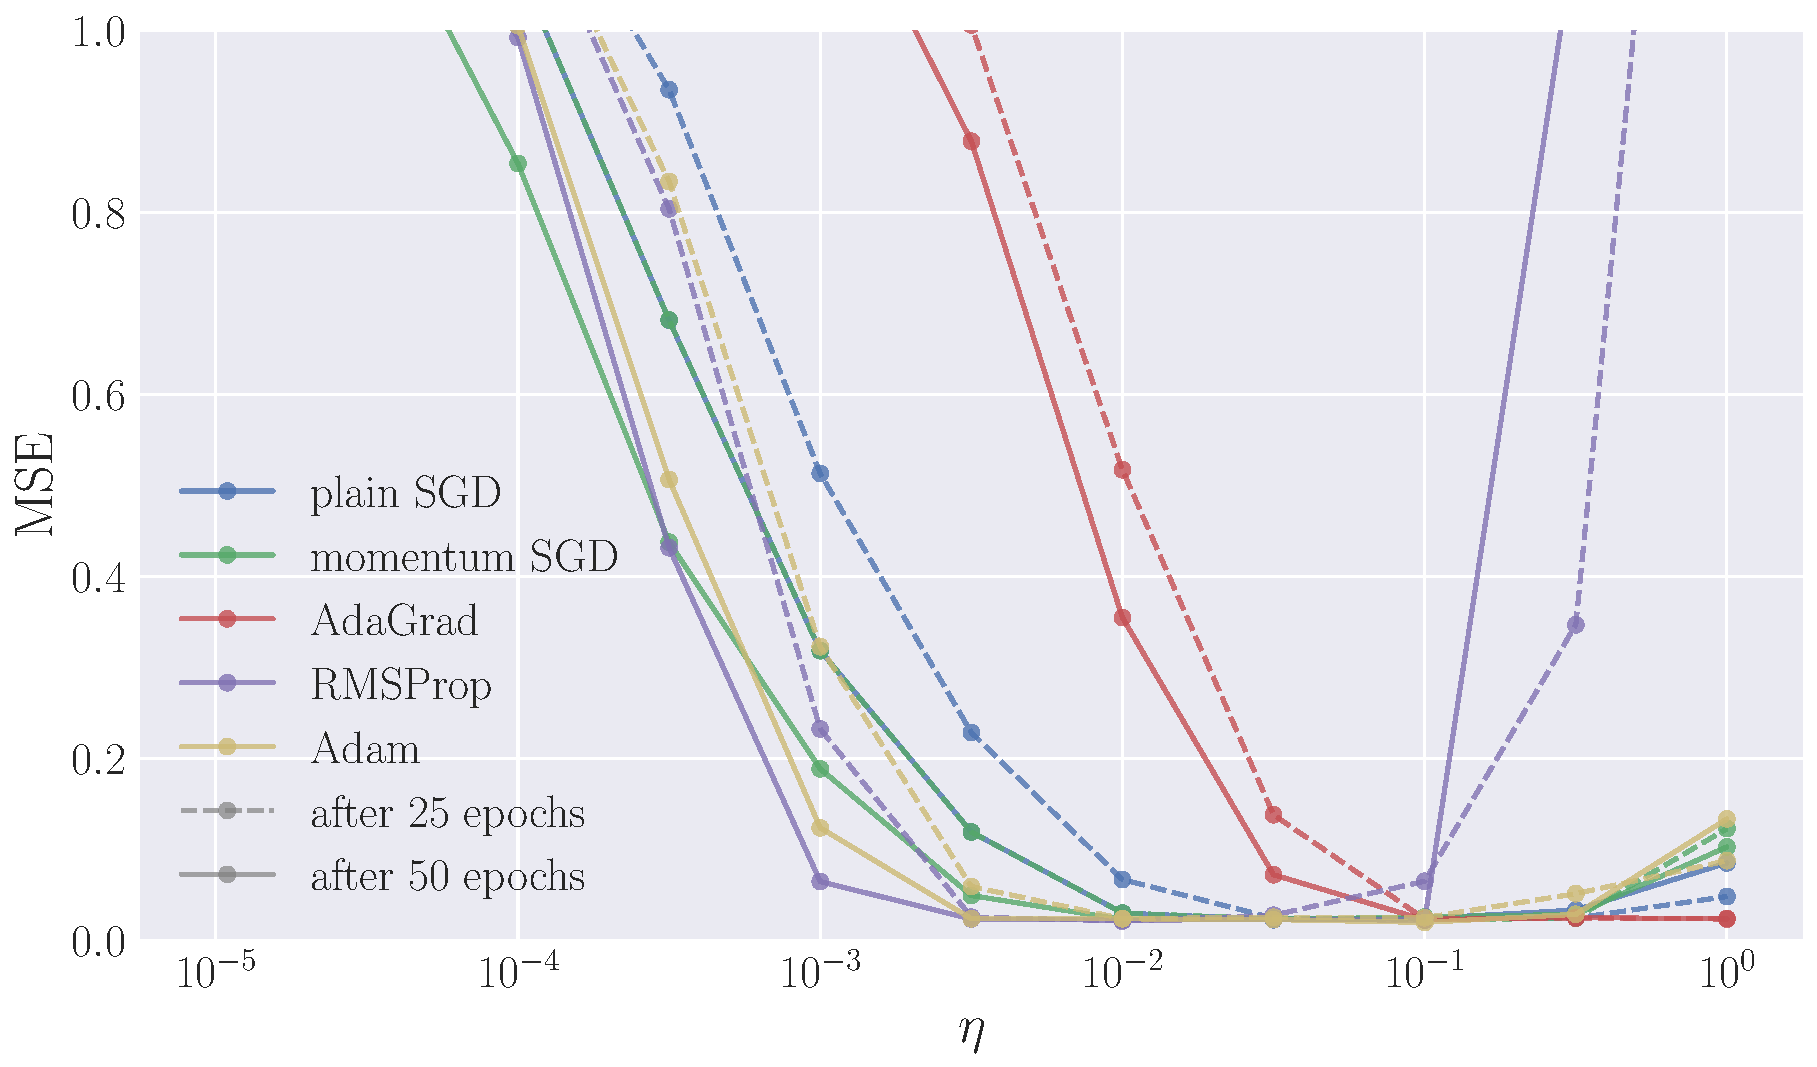
\includegraphics[width=\linewidth]{ridge_errors_gradient_descent.pdf}
        \caption{The graphs show how the test MSE evolves as the global learning rate $\eta$ increases for different update rules in the SGD algorithm. The penalty parameter is $\lambda=0.1$, and we have used $m=40$ minibatches. $\gamma=0.5$ for the momentum SGD and the other relevant hyperparameters are set to their defaults in accordance with section \ref{sec:tuning}. The dashed graphs show the MSE after 25 iterations and the solid graphs represent the MSE after 25 additional iterations. All solvers were initialised by the same random vector $\svec{\theta}_0$.}
        \label{fig:simple_reg_errors_ridge}
    \end{figure}

    We will study more thoroughly the dependencies on the number of epochs, the number of minibatches ($m$) and the penalty parameter ($\lambda$) in the NN analysis of the Franke function in section \ref{sec:analysis_NN}. 

    
\subsection{Neural network}\label{sec:analysis_NN}
    We will build our FFNN (\ref{item:prepocess}-\ref{item:optimiser}) and solve a supervised learning problem (\ref{item:train}-\ref{item:review}) using the steps listed below \citep{mhjensen}.

    \begin{enumerate}[label=(\roman*)]
        \item\label{item:prepocess} Collect and prepocess data, that is we extract 80\% of the dataset and reserve the rest for validation. The data is then scaled using standard score normalisation\footnote{Formula found in \cite{mhjensen}, or page 6 of the \projectOne-report.} with respect to the training data.
        \item\label{item:architecture} Define the model and design its architecture. In practice, this means to decide on hyperparameters of the NN such as depth ($L$) and activation function(s) ($g$).
        \item\label{item:optimiser} Choose loss function and optimiser. For regression we will use the MSE score \eqref{eq:linear_regression_cost_function} as the estimator of loss, whereas the classification problem estimates the loss according to the cross entropy \eqref{eq:logistic_regression_cost_function}. We will use SGD as optimiser, but we have various alternatives for the exact optimisation algorithm (see section \ref{sec:tuning}).
        \item\label{item:train} Train the network to find the right weights and biases.
        \item\label{item:assess} Validate model, i.e. assess model performance by applying it on the test data.
        \item\label{item:review} Adjust hyperparameters, and if necessary review the network architecture. That is to say, if the result is not satisfactory even after tuning the hyperparameters, return to step \ref{item:architecture} and start over from there. 
    \end{enumerate}

    %In practice, the steps \ref{item:architecture}-\ref{item:review} will be performed several times 
    

\subsection{Regression problem}\label{sec:analysis_regression}


    Our dataset is once again fictional as it is generated by the Franke function from \projectOne\footnote{Equation (10) in the report.} with an added noise of $0.1 \mathcal{N}(0, 1)$ for a set of coordinates in the plane. We split and standardise the $20\times 20$ data points, which concludes step \ref{item:prepocess}. 
    Eventually we want to optimise the network architecture. However, in order to begin generating result we need an initial architecture that is not too computationally expensive, but yet versatile. We initialise the network with 3 hidden layers with 15, 10, and 5 neurons each, result in depth of $L=4$. We begin our analysis with the sigmoid function as activation function for the hidden layers and a linear output function. We use SGD with RMSProp as our optimiser of choice, dividing the training data into 3 minibatches. This concludes step \ref{item:architecture} and \ref{item:optimiser}.
    We then train our network for 250 epochs, which at this stage is a fair trade off between computational efficiency and fine tuning of the network. The trained model is tested against the test data and performance is recorded. 

    Now that our network is set up we are ready to test it. The first task is to determine the hyperparameters $\eta$ and $\lambda$ given the architecture above. From figure \Fig{reg_eta_lambda} it is obvious that the current choice of architecture and training prefers relatively large learning rates and small regularisation parameters. The large error for smaller learning rates is most likely due the number of epoch being too small for these learning rates to find the minimum of the loss function. For now this result is satisfactory and we note the optimal parameters to be $\eta=10^{-1}$ and $\lambda=10^{-4}$. 

    Now we take a closer look at the architecture of the network and perform analysis of a model where we increase the number of hidden layers $L-1$ with a fixed, but increasing number of neurons per layer $N_l$. \Fig{reg_layer_neuron} show the results, where it becomes apparent that for the optimal parameters mentioned above, a network with a simple architecture (few layers and neurons) is preferred with the optimal architecture being a network with one hidden layer that contains 30 neurons. The mean squared error is steadily decreasing, and we note the current value to be $\mathrm{MSE} = 0.057$. 

    The next thing to decide is the activation function of the hidden layer. In \Fig{reg_act_epoch1000} and \Fig{reg_act_epoch} we have plotted the MSE as function of training epochs, for up to 1000 and 250 epochs respectively. For computational efficiency we want to train the network for as few epochs as necessary, but we should also check how increasing the training epochs affect the performance of the model. From these two figures we draw that the sigmoid and and hyperbolic tangent activations show the most promising results, with sigmoid being the most stable. Hence, we use sigmoid when performing the final analysis. In addition, we do not expect the model to perform significantly better if we increase the number of epochs. We also note the stochastic behaviour of the graphs, except for the ReLU graph. This could be since ReLU have the ability of killing neurons when its derivative is zero. 

    Having a model we need to decide on the best way of training it. \Fig{reg_minibatch_epoch} shows a heatmap of the number of epochs against the number of minibatches. Few minibatches and few epochs result in computational efficiency. However, there does not seem to be an overall preference. We therefore choose the best value of those presented and train the model over 700 epochs using 2 minibatches. 

    The final model consist of a network with one hidden layer that contains 30 neurons. The learning rate and regularisation is tuned to be $\eta=10^{-1}$ and $\lambda=10^{-4}$, where we use sigmoid as the activation function of the hidden layer. The model is trained over 700 epochs using 2 minibatches. This results in a test MSE of 0.052, which is significantly less than 0.15 as we got with normal OLS analysis in \projectOne. In order to validate our model we let the model fit a function to the original noise Franke function data. The result is shown in figure \Fig{franke}, where the data points are shown with green triangles. As is visible in the figure, the model does quite a decent job of fitting this function to the data points for the given domain. 

    \begin{figure}[h!]
        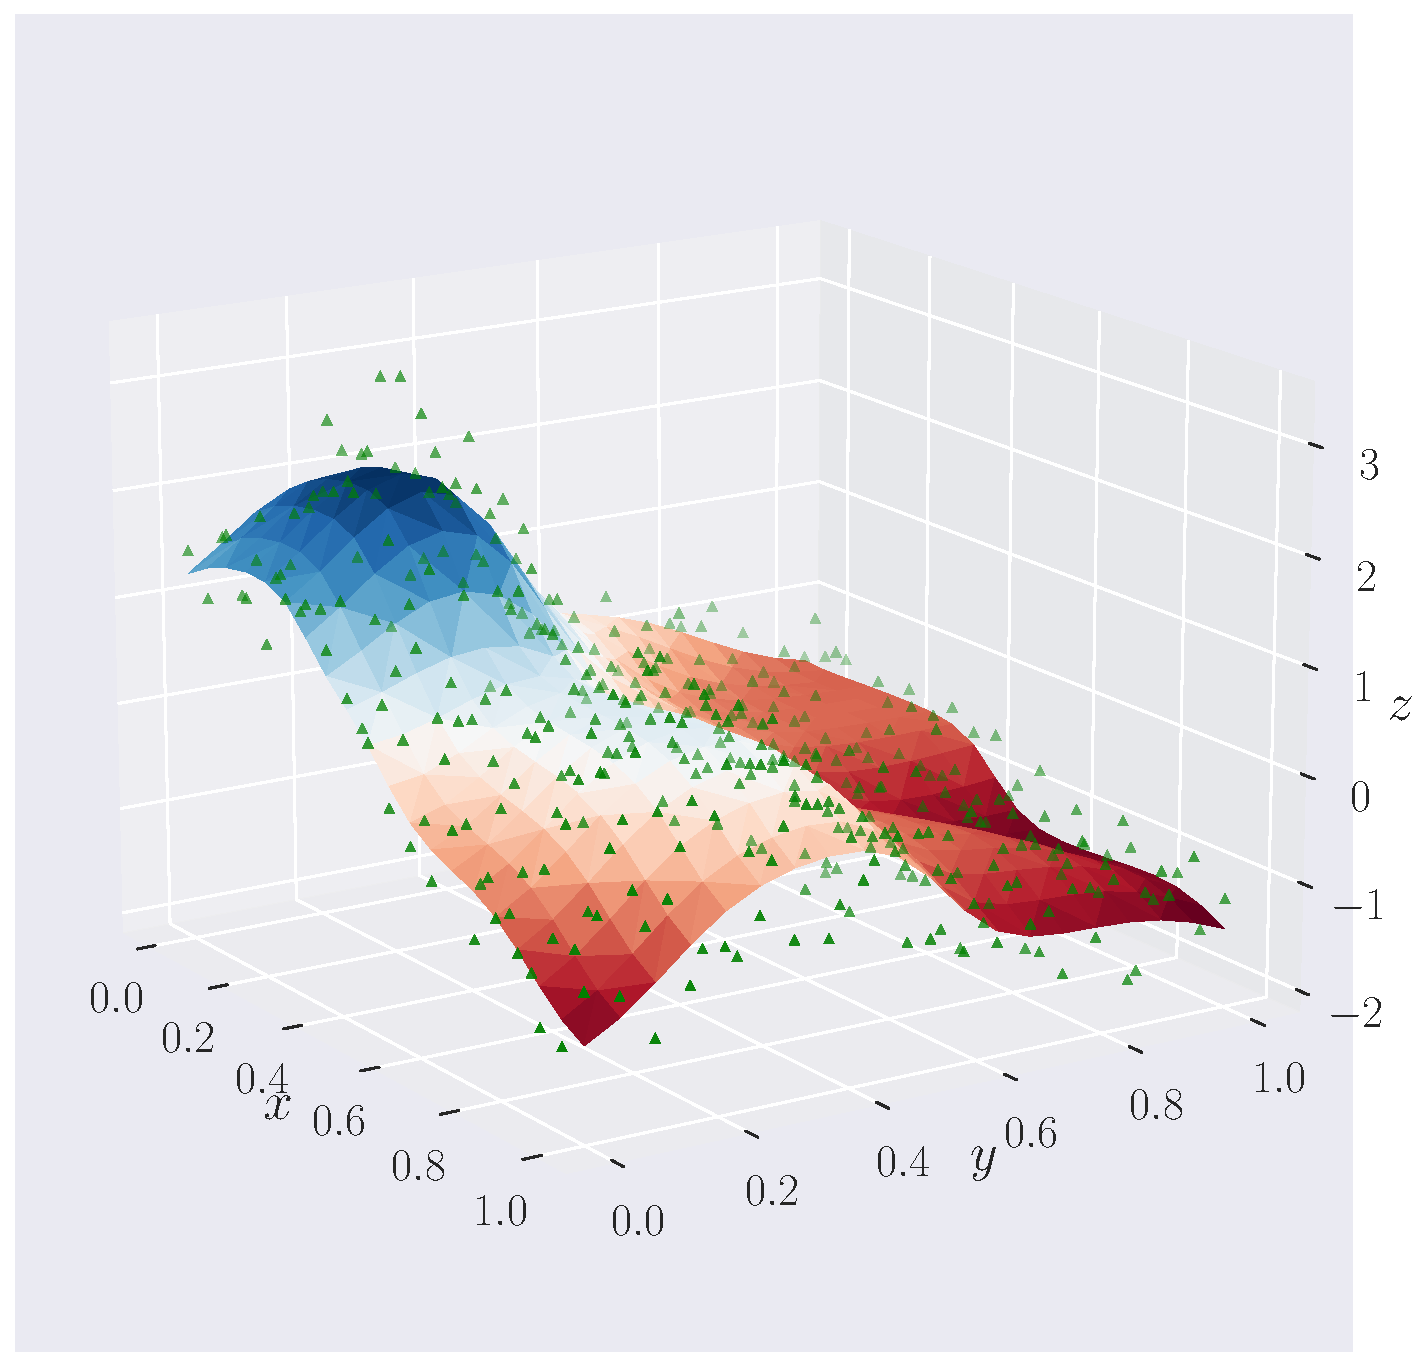
\includegraphics[width=\linewidth]{franke.pdf}
        \caption{Best fit of the Franke function (original data shown with green triangles). The model used has 1 hidden layer with 30 neurons, $\eta=10^{-1}$, $\lambda=10^{-4}$, with a sigmoid activation function trained for 700 epochs with 2 minibatches. This resulted in a test MSE of 0.052}
        \label{fig:franke}
    \end{figure}

    It is perhaps surprising that the ReLU and leaky ReLU activation functions perform so badly. One could expect that these activation function should outperform the sigmoid and hyperbolic tangent activation function. Reason for the results obtained here could very well be implementation errors in the model and initialisation. In addition, the order in which we test and decide hyperparameters should perhaps also play a role. If we revert the order and say, start with a given $\eta$ and $\lambda$ and tune the architecture before tuning the hyperparameters the result could have been different. There are numerous ways of testing and deciding on parameters for such a network, and the procedure presented here is just one of many possibilities. In the end, the MSE obtained is lower than what we found for OLS, which is a satisfactory result. Also, proposed ideal architecture is not computationally expensive and simulations are thus easy to run. 

  






\subsection{Classification problem}\label{sec:analysis_classification}
    For the classification problem we use the Wisconsin Breast Cancer dataset provided by Scikit-learn \citep{scikit-learn}. In short, this dataset consists of 569 samples, each with 30 features, divided into 2 classes; those that were benign, and those that were malignant. This is thus a \textit{binary classification problem} due to the two classes. The major differences to our network model will be the number of input neurons, which will now be 30 (features), and a single output neuron with a sigmoid output function. We will also use cross entropy, \Eq{logistic_regression_cost_function}, as our loss function. 
    
    For comparative reasons, we perform the analysis in a similar manner as with linear regression, and we start with the same model architecture; a network with 3 hidden layers, with 15-10-5 neurons in each layer. We minimise the loss function in the same way, using SGD with RMSProp as our chosen optimiser algorithm, starting with 3 minibatches. From \Fig{class_eta_lambda} with find the optimal hyperparameters to be $\eta=10^{-3}$ and $\lambda=10^{-6}$. From figure \Fig{class_layer_neuron} we find the the optimal architecture, given the hyperparameters is a network with 2 hidden layers, each with 10 neurons. We also note that in this case there is no significant favourisation of the simpler networks, as it was for linear regression. However, we choose the simplest one, with the highest accuracy. \Fig{class_act_epoch1000} and \Fig{class_act_epoch} show the accuracy as function of training epochs for the four different activation functions, given the above architecture. We see that the accuracy when using ReLU is close to 1, when we increase the training epochs, and we deem this to be the optimal activation function. With the above conditions, the optimal model should be trained for 900 epochs using 5 minibatches according to figure \Fig{class_minibatch_epoch}, which gives an accuracy of 1\footnote{Given to two significant digits, which would allow for a few false predictions given the size of our dataset}.

    The difficulties of finding an optimal model for a classification problem are similar to those of classification. The above architecture and tuning is only one of many ways of designing a model which would yield good results. It is difficult to be adamant that one model outperforms the others, since we have only tested for one, and also because the way we decide on the architecture and parameters could very well be switched around. Even for the model at hand, the heatmaps does not give a definite answer as to which set of hyperparameters or architecture is actually best, only how good they are. It is therefore wise to choose the simplest solution  (most computationally efficient) that yield the most accurate result. However, the model at hand gives a descent result, and seem to work well.

\subsection{Logistic regression}\label{sec:analysis_logistic_regression}
    When performing the logistic regression analysis we notice that this is equivalent of having a neural network with no hidden layers and sigmoid as activation function. We use SGD with RMSProp as optimiser, so the only parameters we need to determine are the learning rate and regularisation. We use 250 epochs and 3 minibatches. From \Fig{logistic_eta_lambda} we have that the optimal hyperparameters are $\eta=10^{-3}$ and $\lambda = 10^{-8}$. The obtained accuracy is 1\footnote{Again, to 2 significant digits, which may contain a few false predictions}, which is satisfactory. We are thus pleased with this model and can deduce that it performs as well as the tuned neural network. 

\subsection{Closing words}\label{sec:analysis_closing_words}
There are three appendices to this report, all of which \rephrase{stuffed} with figures supporting our analysis.
    We have so far given estimates of how good our models are in terms of generalisation MSE and accuracy based on an untouched part of the dataset. There are more bulletproof ways of giving these measurements, for instance the bootstrap or cross-validation methods we discussed in \projectOne. Especially alarming are the accuracy scores of 1, which in reality is not realistic. An FFNN such as ours should not give such perfect results, however, we know that the classification dataset we use is ideal for such analyses. That is to say, there is most likely a single feature (or maybe a several few) that discloses whether a person has cancer or not. That would be plain to see if we were to make a histogram the frequency of said feature(s) where we separate the malignant cases from the benign cases and see if they overlap at all. If they do not or only a little, then this would be a very important feature. In any case, we might have benefitted especially in this case from using some resampling methods.

    In this analysis, we have favourised RMSProp as optimiser. \fillertext[Something about why]
\section{Conclusion}

\section*{Code availability}
The code is available on GitHub at \url{\projectTwolink}.

%\newpage
%\listoffigures

\bibliography{ref}

\clearpage



\appendix

\section{Regression figures}\label{app:regression}

\begin{figure}[h!]
    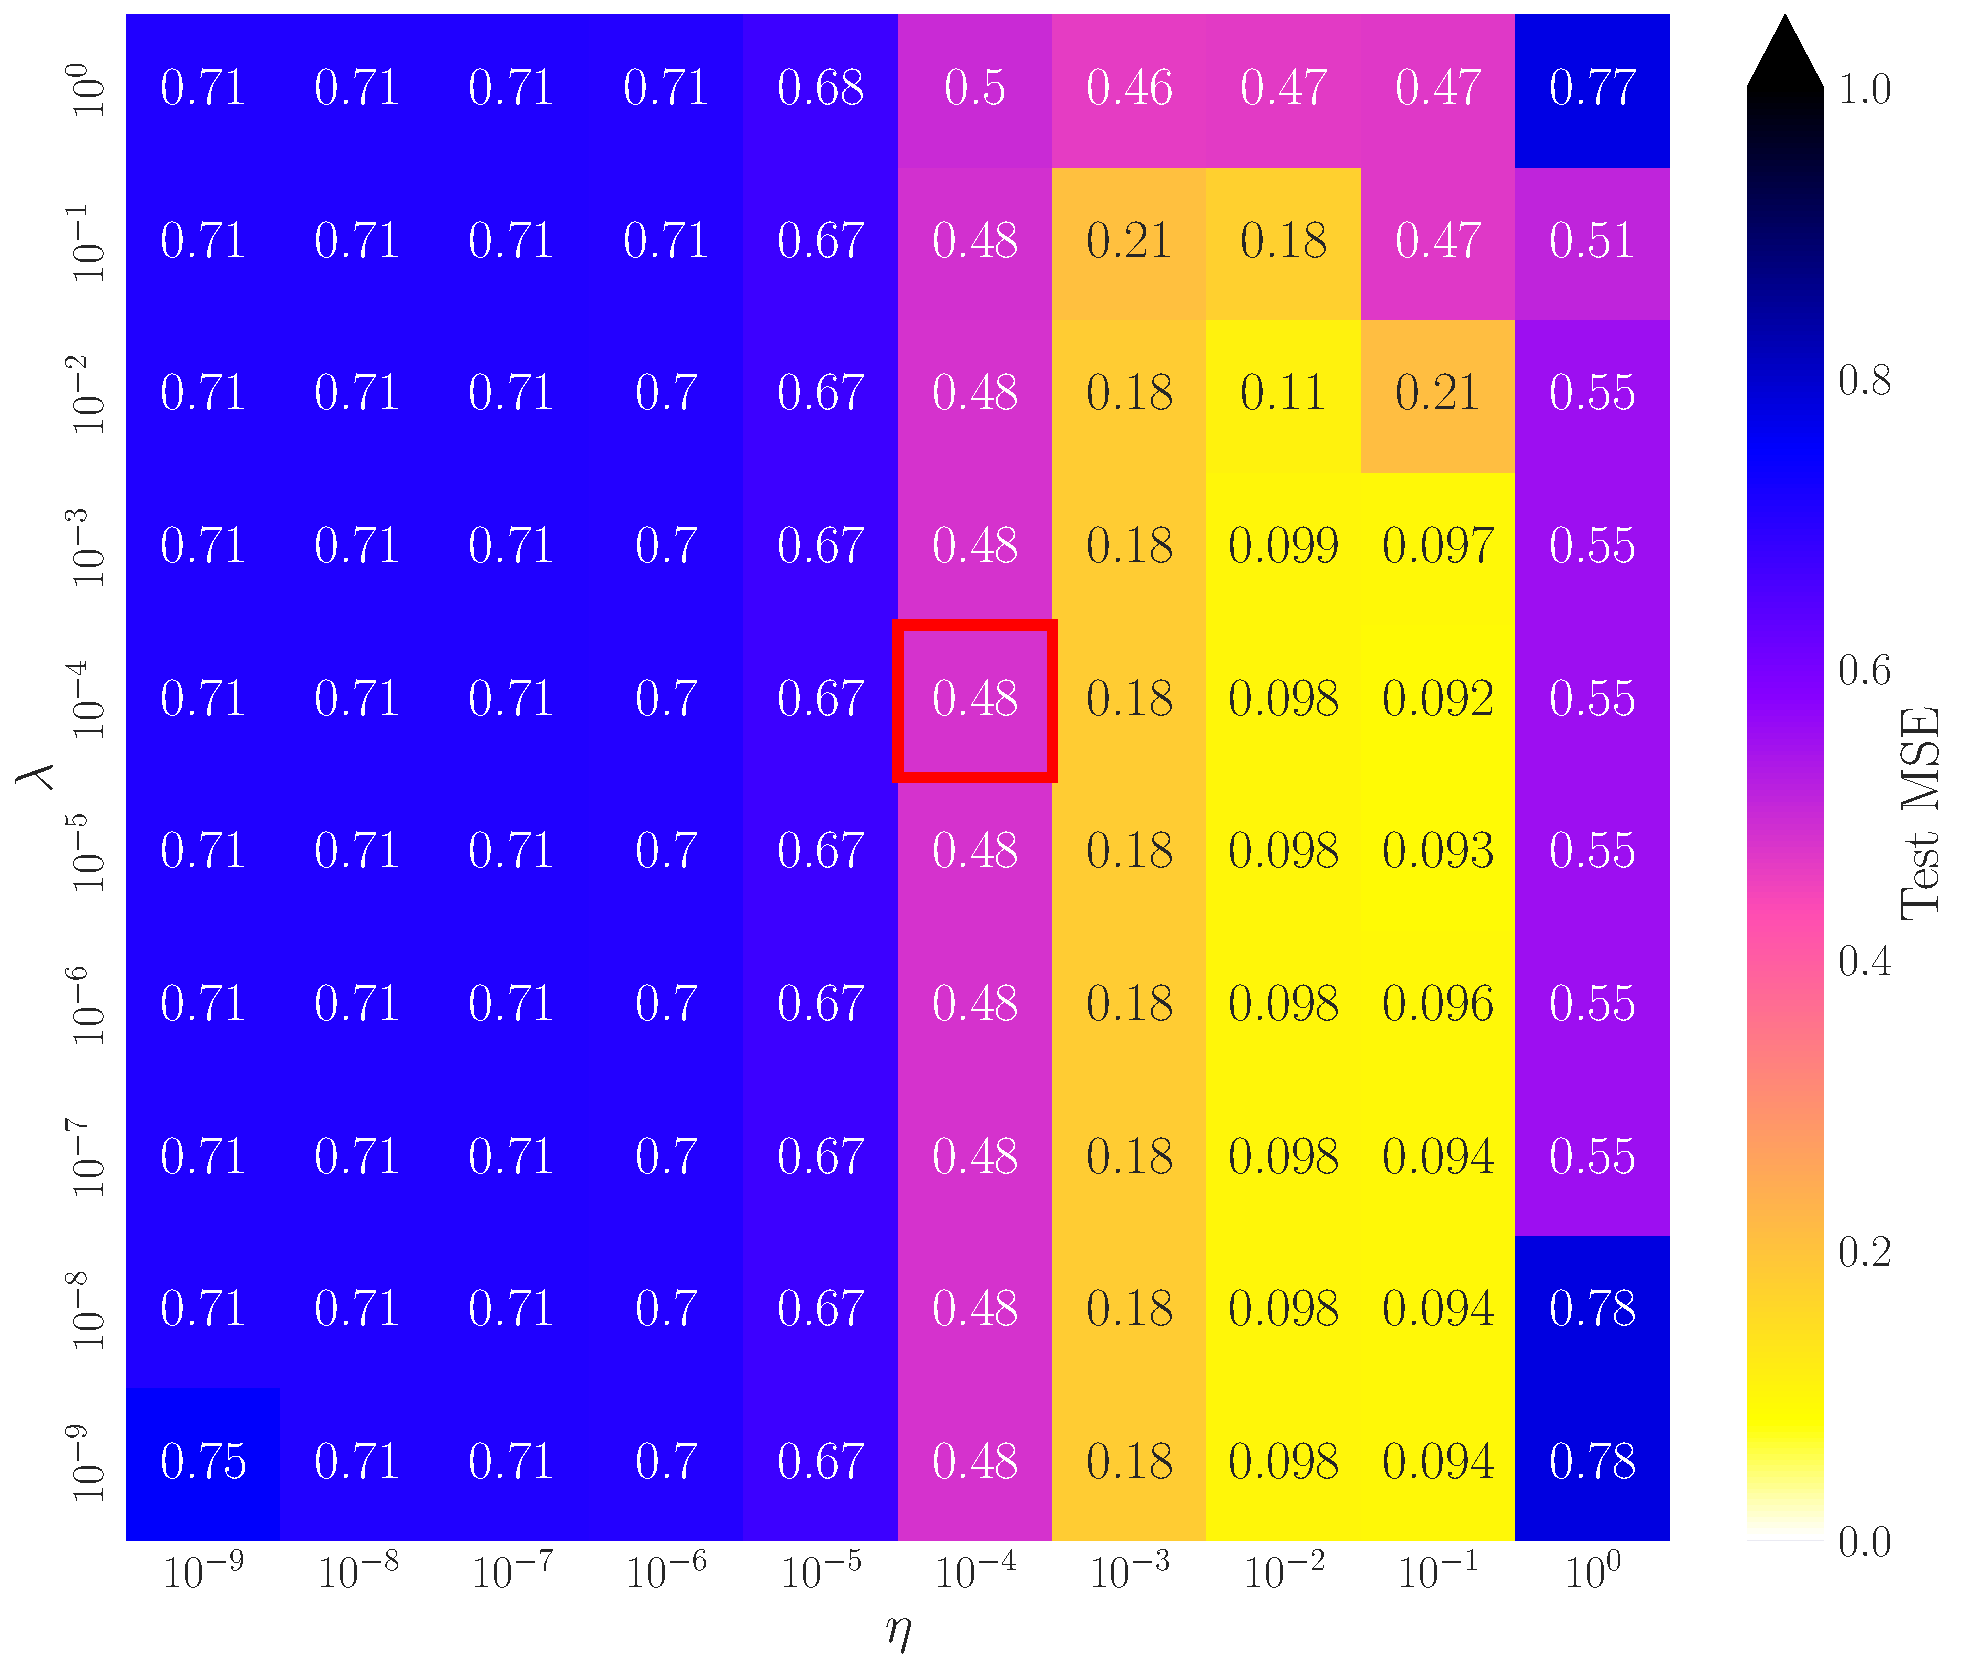
\includegraphics[width=\linewidth]{eta_lambda_analysis.pdf}
    \caption{Heatmap of the MSE as function of learning rate $\eta$ and regularisation parameter $\lambda$, using SGD with RMSProp as optimiser performing regression analysis of a 3 layered, 15-10-5 neurons, neural network. }
    \label{fig:reg_eta_lambda}
\end{figure}

\begin{figure}[h!]
    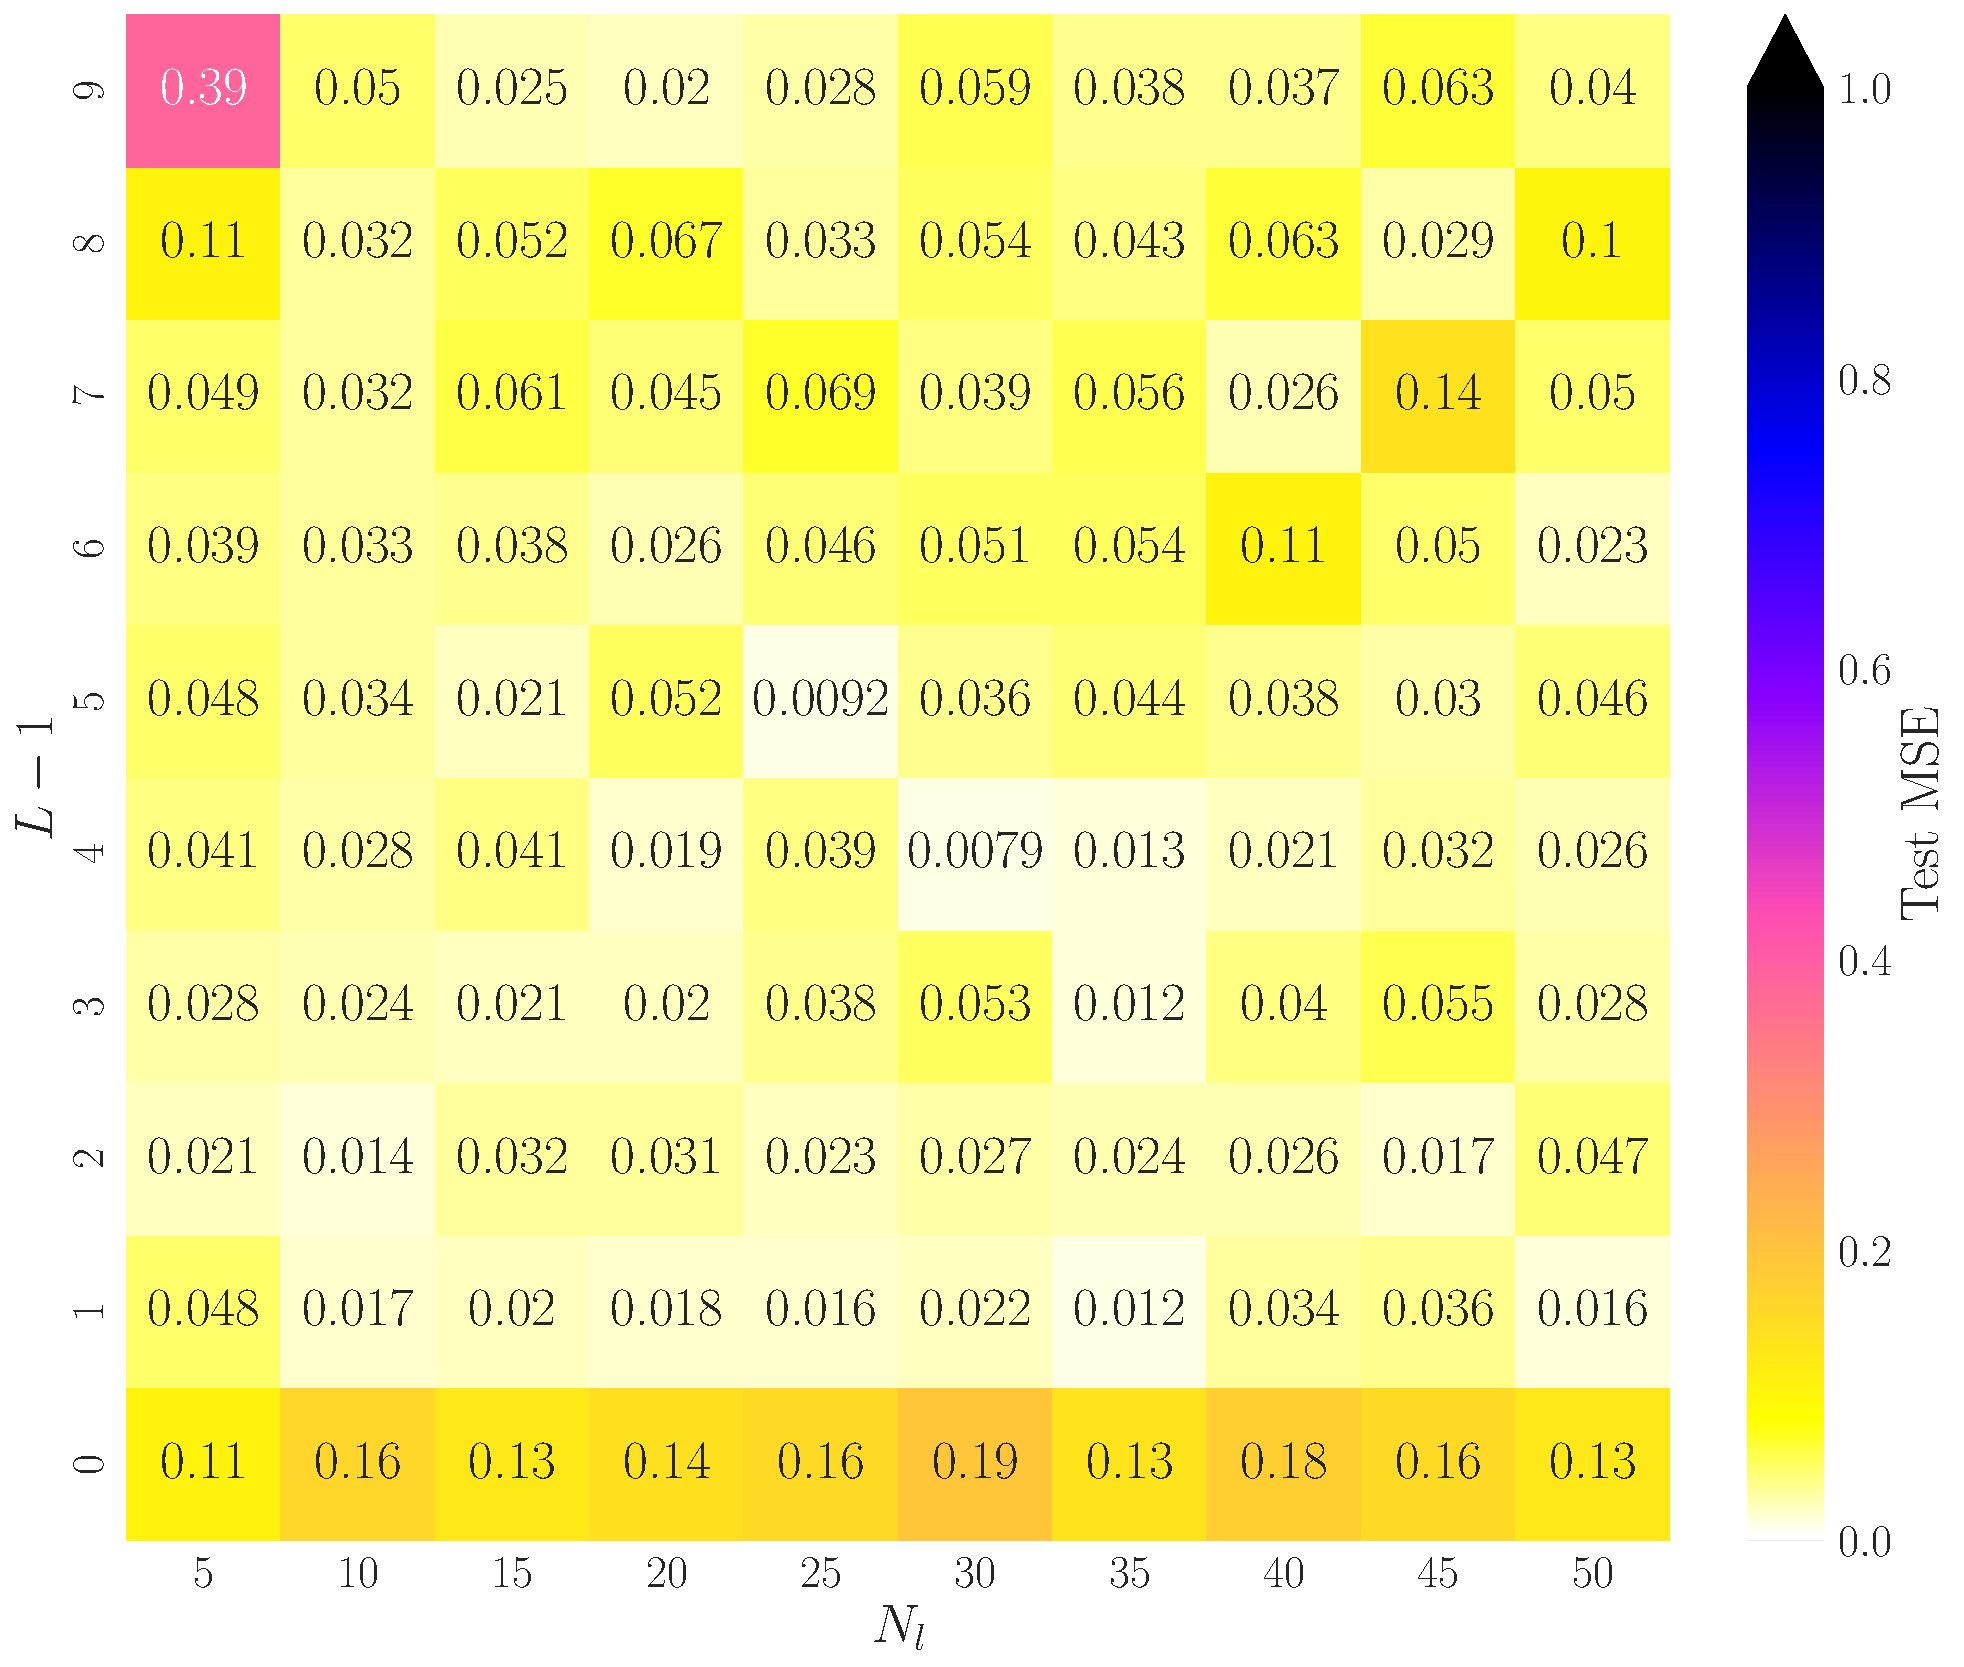
\includegraphics[width=\linewidth]{layer_neuron_analysis.pdf}
    \caption{Heatmap of the MSE as function of hidden layers $L-1$ and neurons per layer $N_l$, using SGD with RMSProp as optimiser performing regression analysis with $\eta=10^{-1}$ and $\lambda=10^{-4}$.}
    \label{fig:reg_layer_neuron}
\end{figure}

\begin{figure}[h!]
    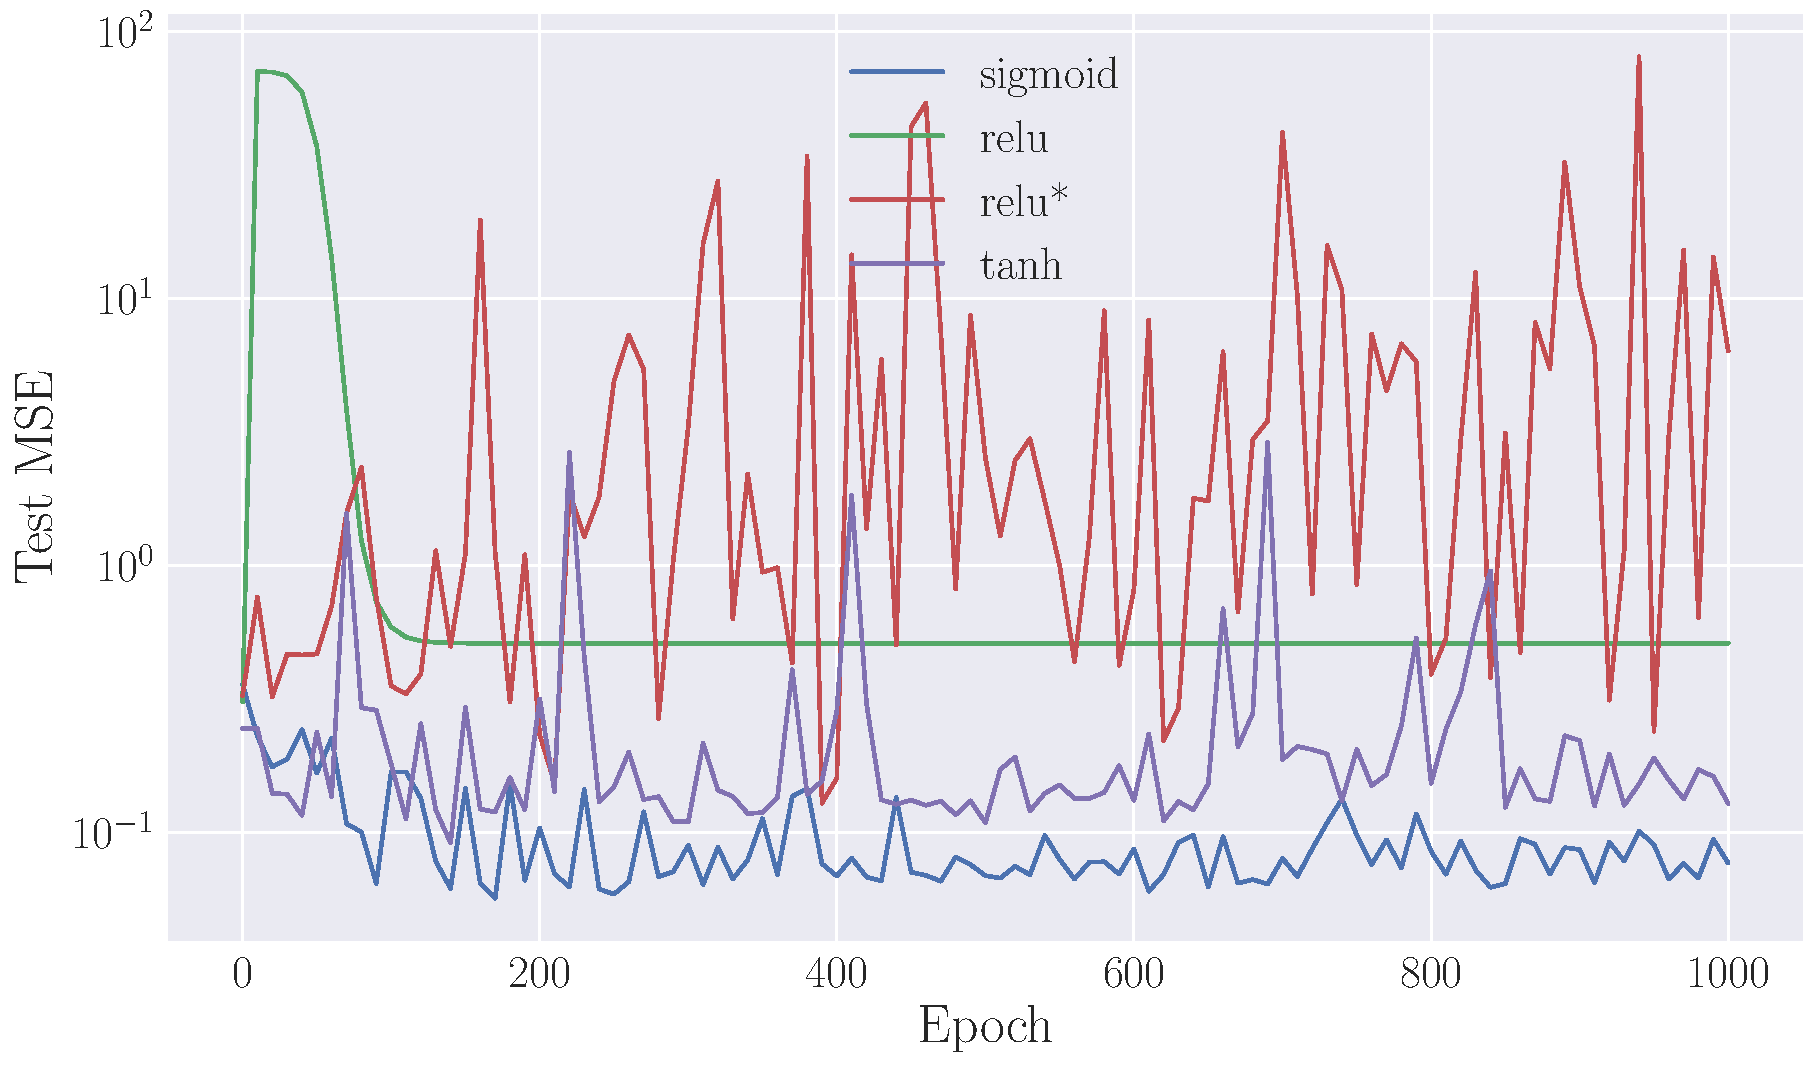
\includegraphics[width=\linewidth]{actFuncPer1000Epoch.pdf}
    \caption{Plot of the MSE for up to 1000 epochs, using SGD with RMSProp as optimiser performing regression analysis with $L-1=1$ hidden layer with $N_l=30$ neurons with $\eta=10^{-1}$ and $\lambda=10^{-4}$. The four different activation functions perform differently. Note the logarithmic MSE axis.}
    \label{fig:reg_act_epoch1000}
\end{figure}

\begin{figure}[h!]
    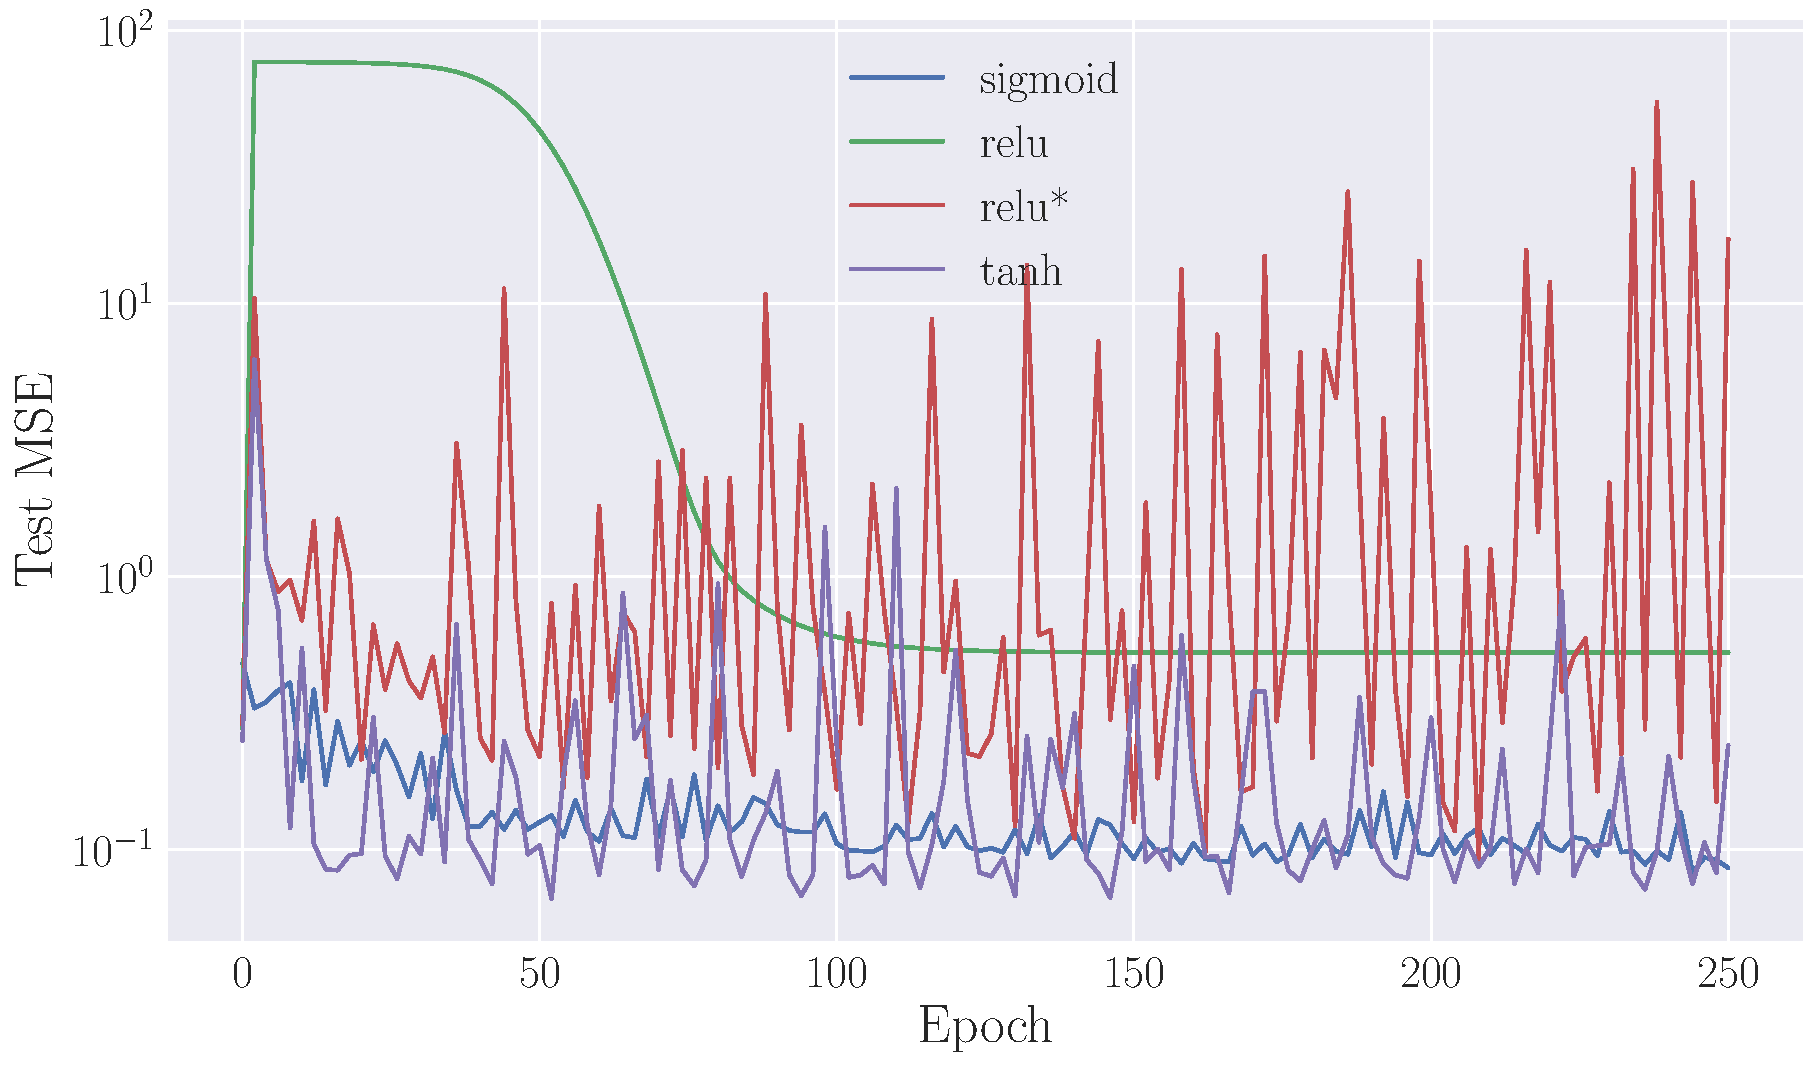
\includegraphics[width=\linewidth]{actFuncPerEpoch.pdf}
    \caption{Plot of the MSE for up to 250 epochs, using SGD with RMSProp as optimiser performing regression analysis with $L-1=1$ hidden layer with $N_l=30$ neurons with $\eta=10^{-1}$ and $\lambda=10^{-4}$. The four different activation functions perform differently. Note the logarithmic MSE axis.}
    \label{fig:reg_act_epoch}
\end{figure}

\begin{figure}[h!]
    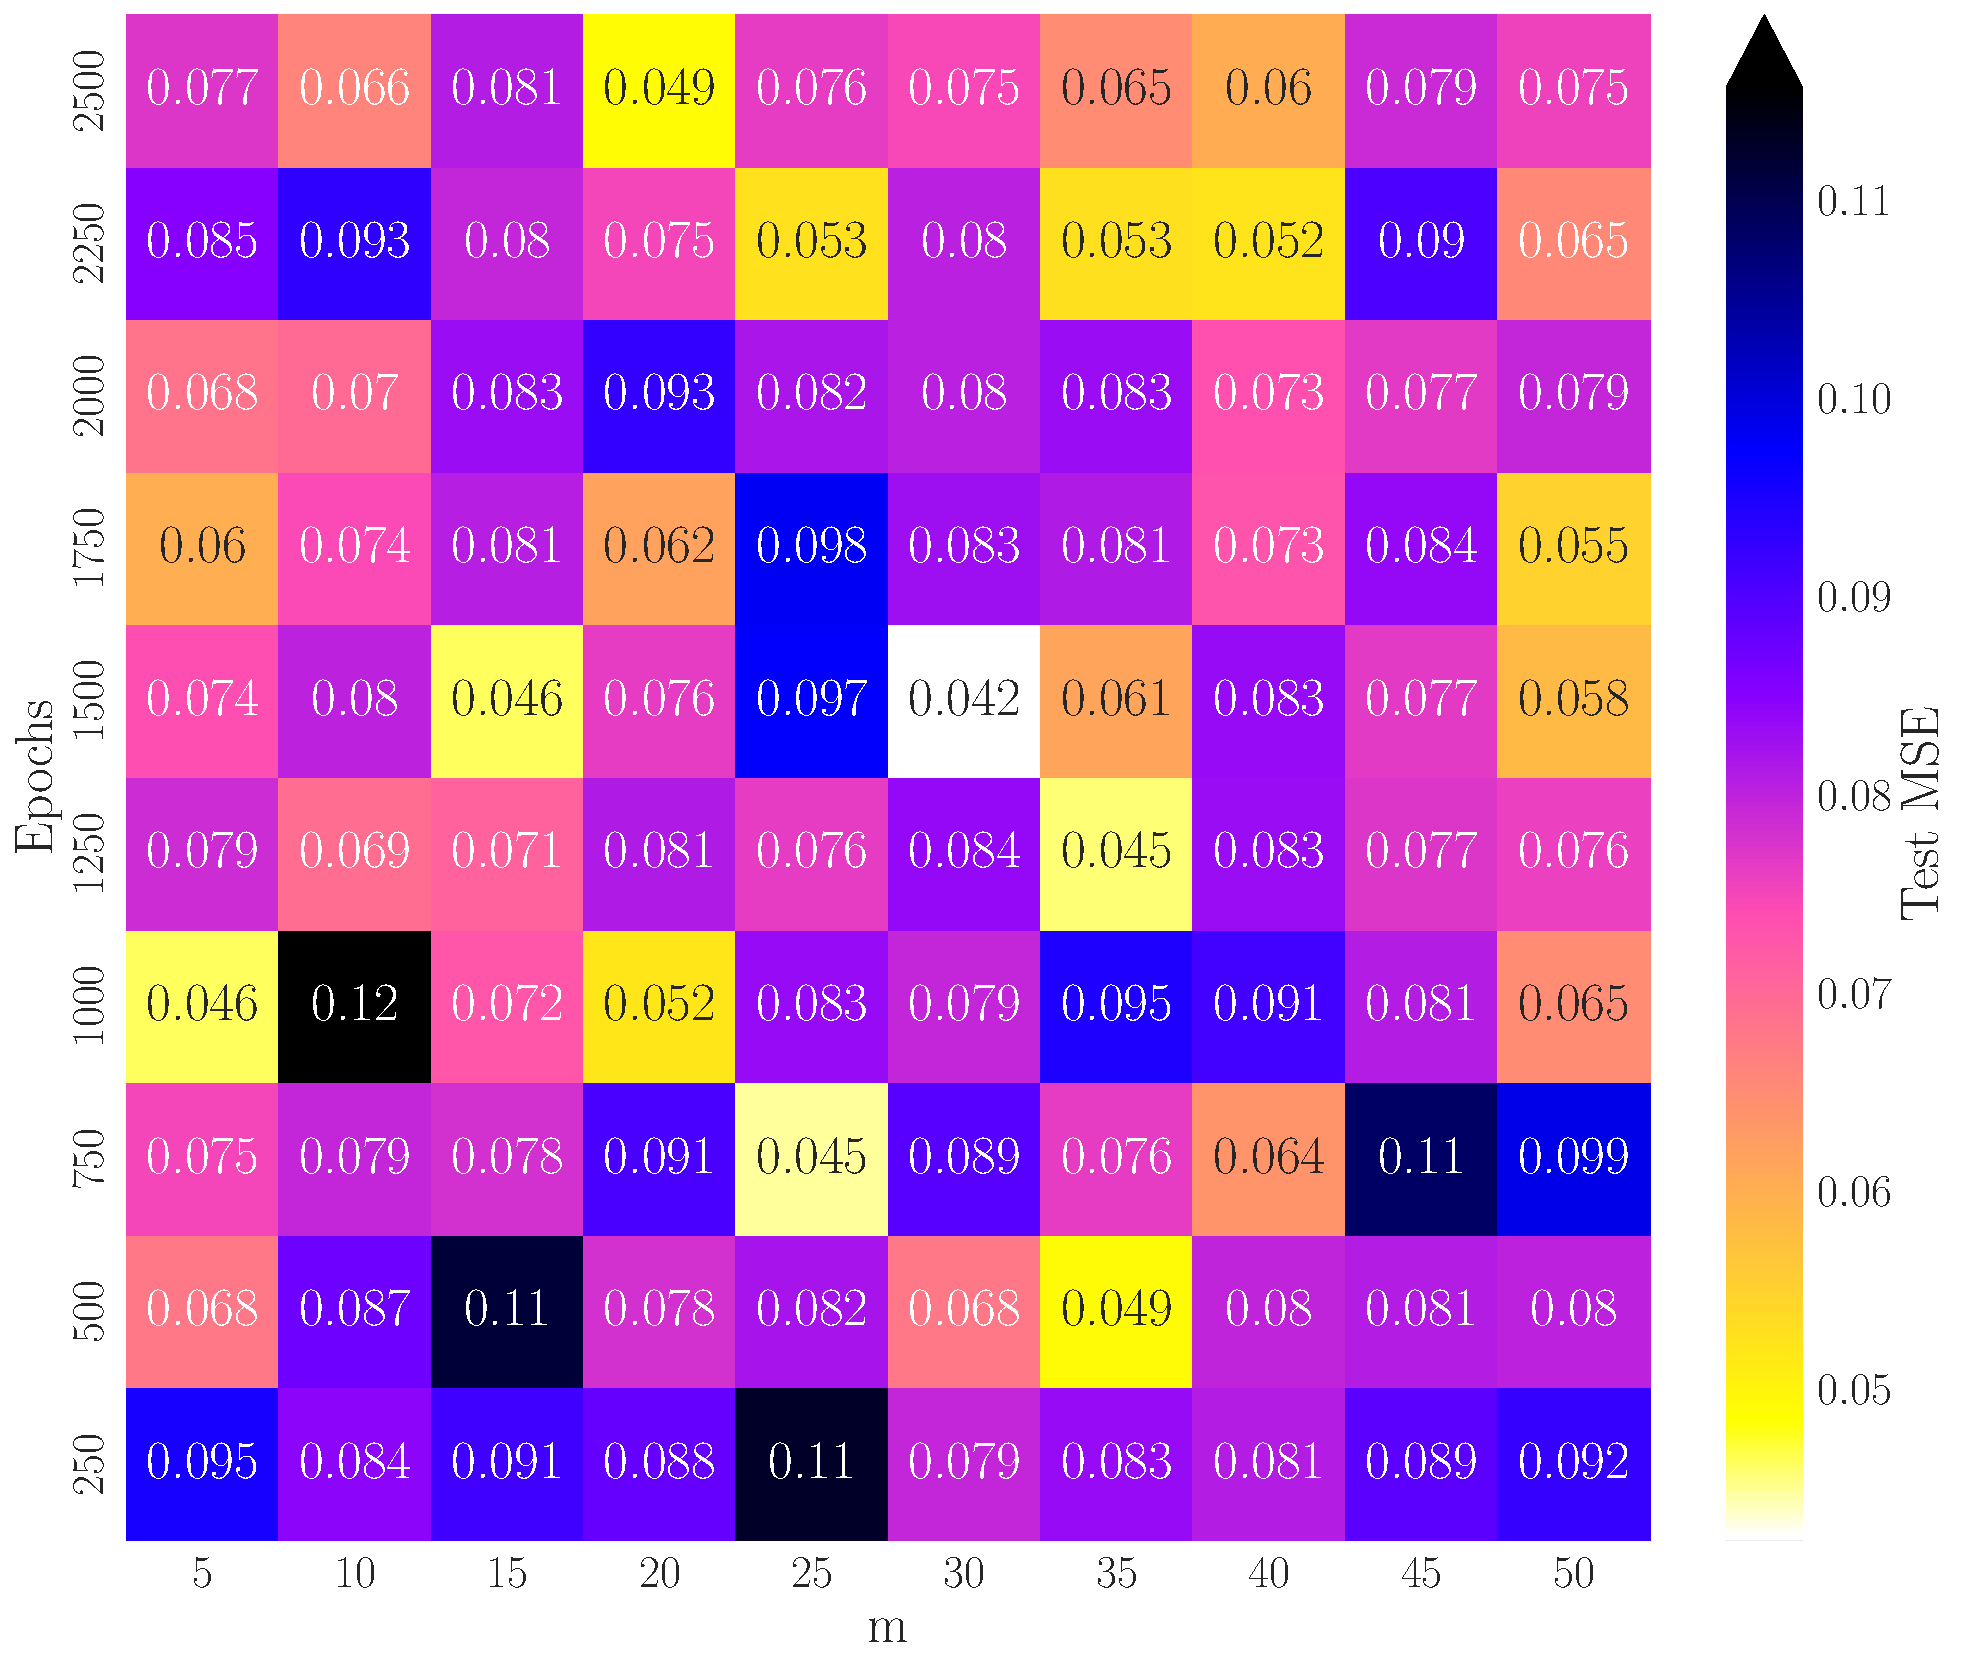
\includegraphics[width=\linewidth]{epoch_minibatch_analysis.pdf}
    \caption{Heatmap of the MSE as function of the number of minibatches $m$ and training epochs, using SGD with RMSProp as optimiser performing regression analysis with $L-1=1$ hidden layer with $N_l=30$ neurons with $\eta=10^{-1}$ and $\lambda=10^{-4}$ using sigmoid as activation function. }
    \label{fig:reg_minibatch_epoch}
\end{figure}




\clearpage

\section{Classification figures}\label{app:classification}

\begin{figure}[h!]
    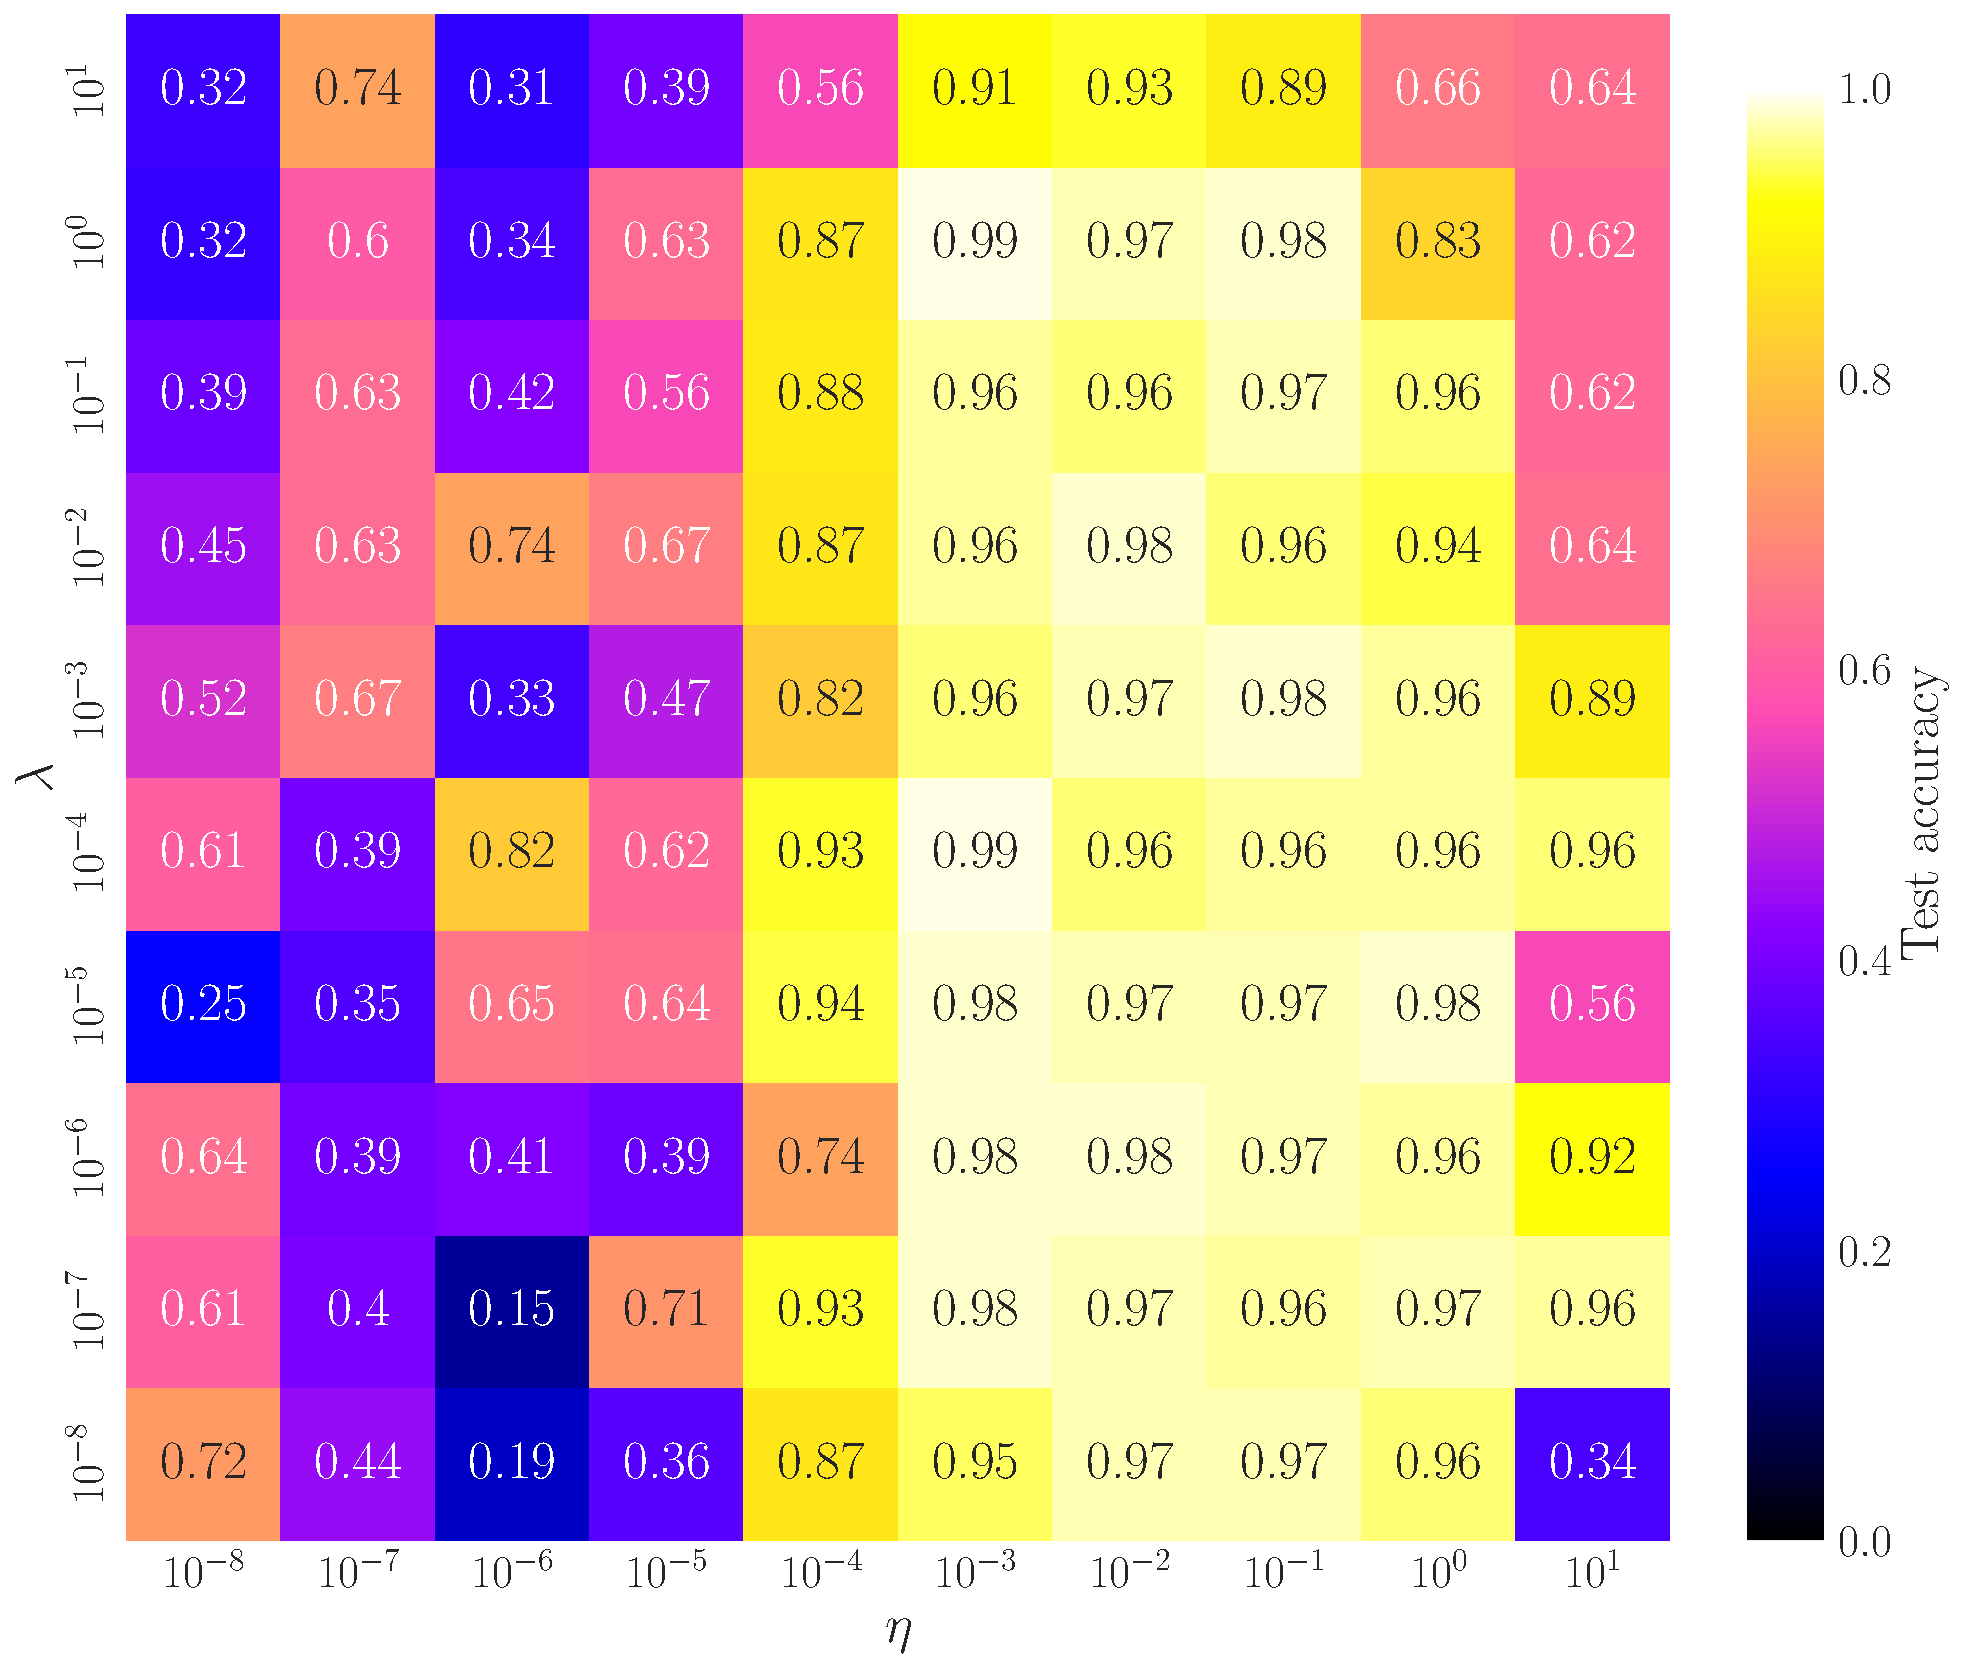
\includegraphics[width=\linewidth]{eta_lambda_analysisCancer.pdf}
    \caption{Heatmap of accuracy as function of learning rate $\eta$ and regularisation parameter $\lambda$, using SGD with RMSProp as optimiser performing regression analysis of a 3 layered, 15-10-5 neurons, neural network. }
    \label{fig:class_eta_lambda}
\end{figure}

\begin{figure}[h!]
    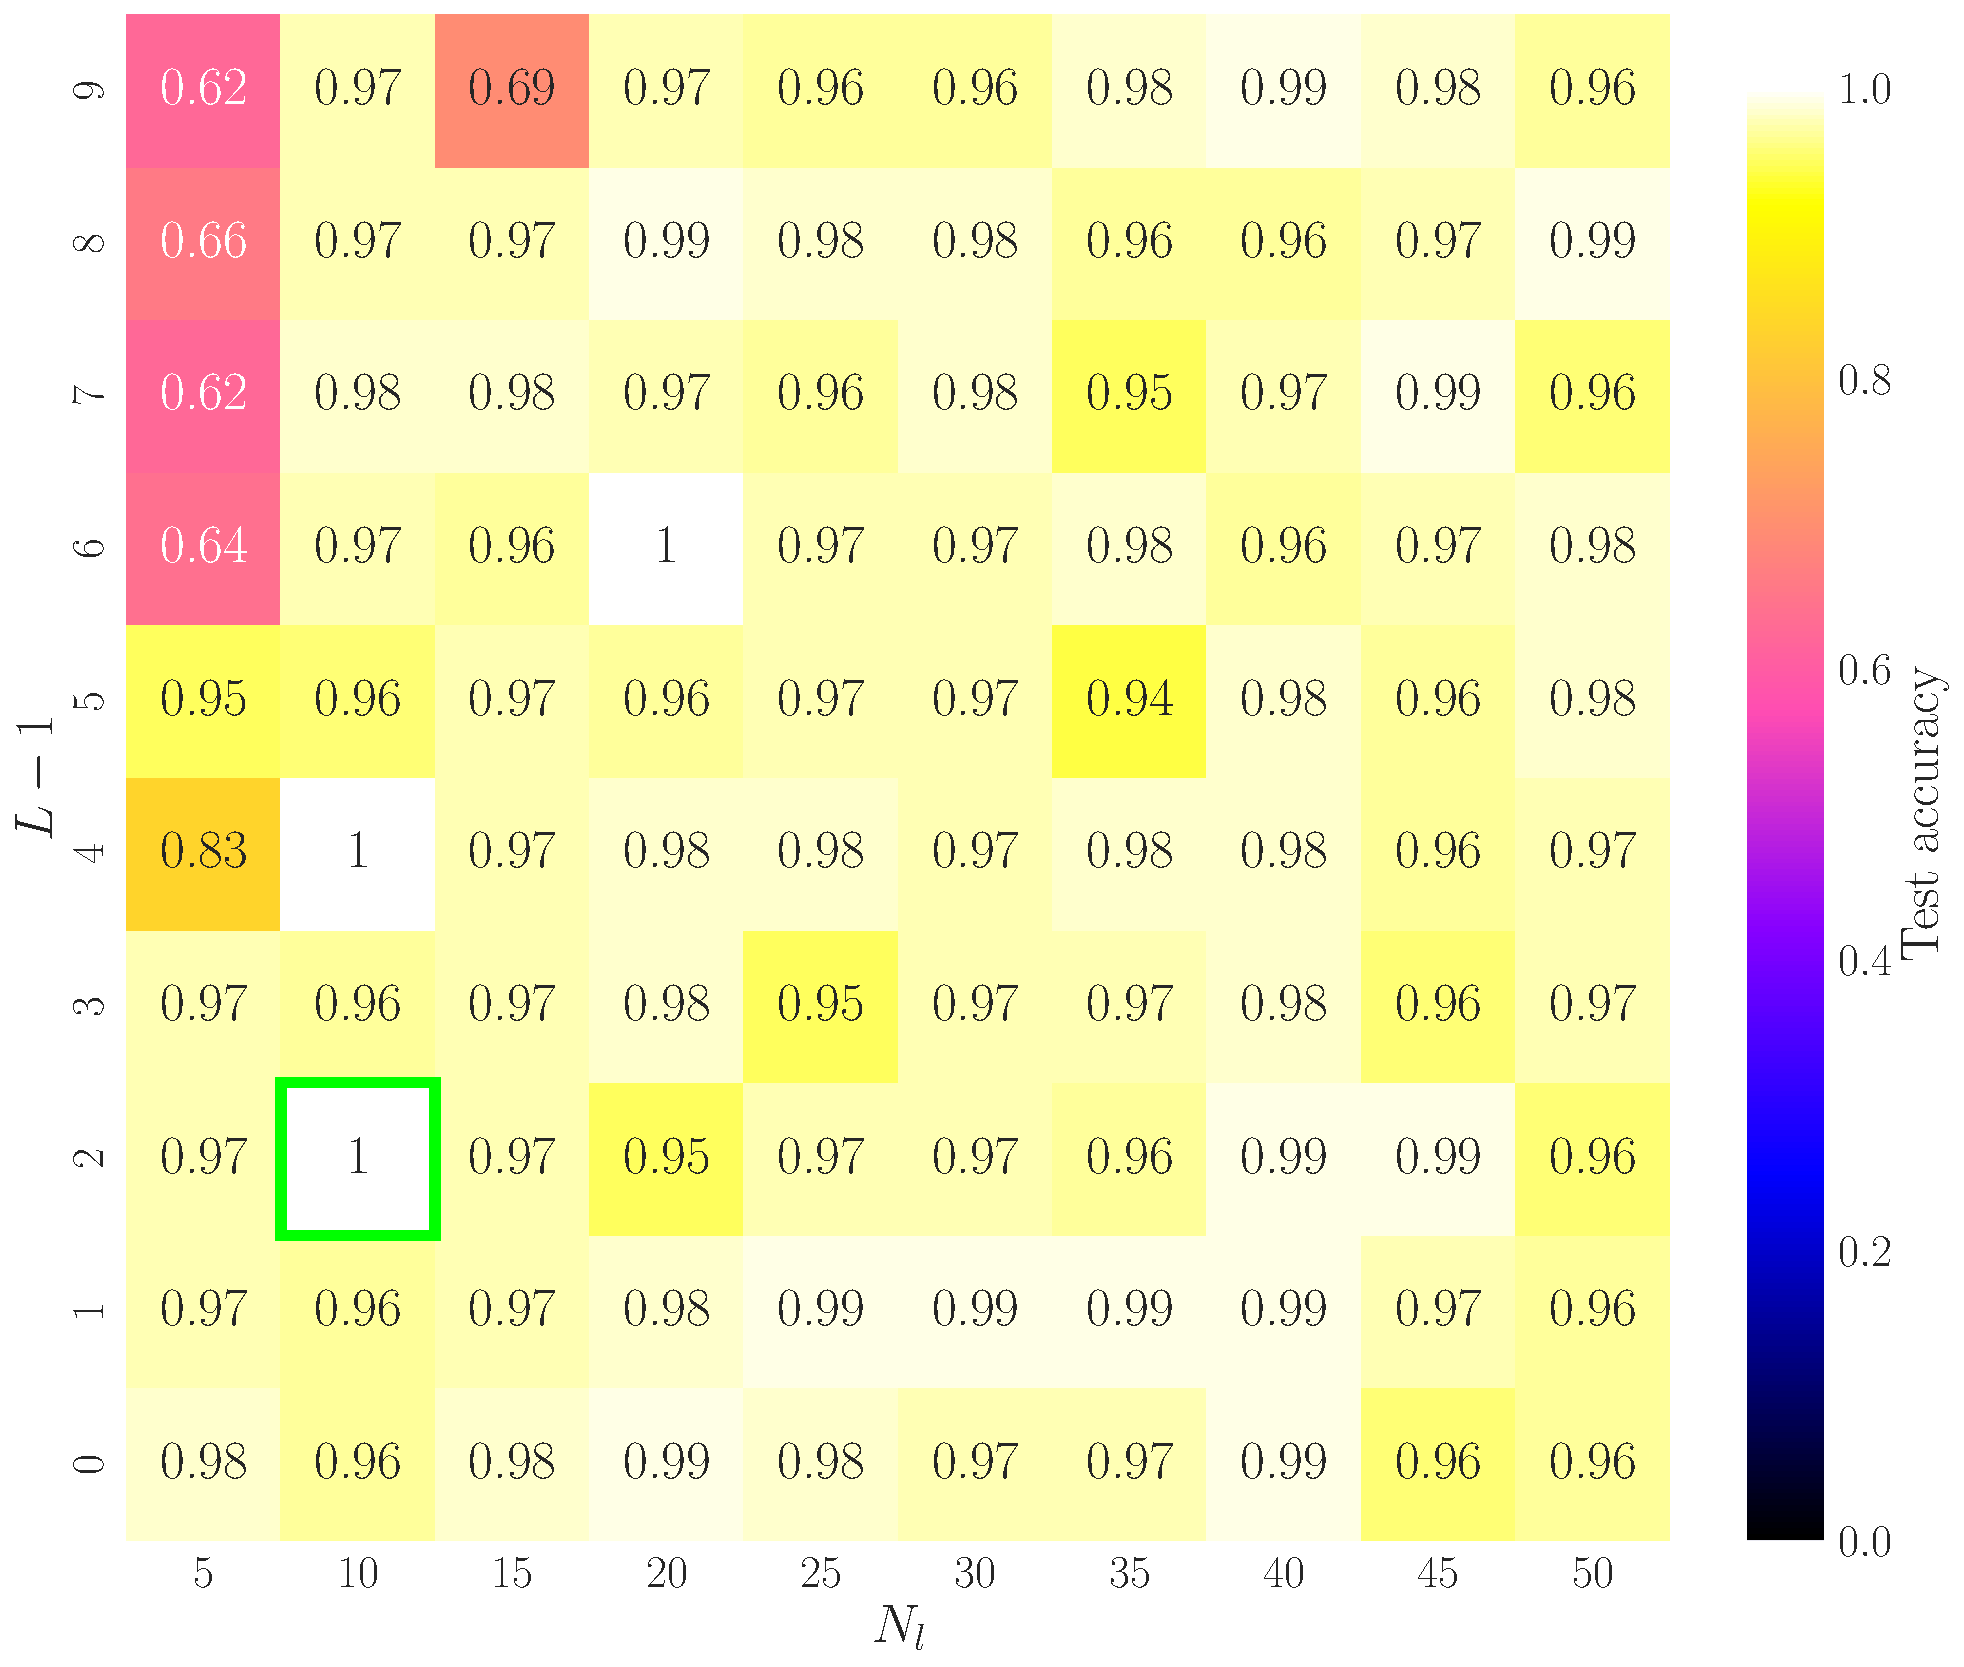
\includegraphics[width=\linewidth]{layer_neuron_analysisCancer.pdf}
    \caption{Heatmap of accuracy as function of hidden layers $L-1$ and neurons per layer $N_l$, using SGD with RMSProp as optimiser performing regression analysis with $\eta=10^{-3}$ and $\lambda=10^{-6}$ }
    \label{fig:class_layer_neuron}
\end{figure}

\begin{figure}[h!]
    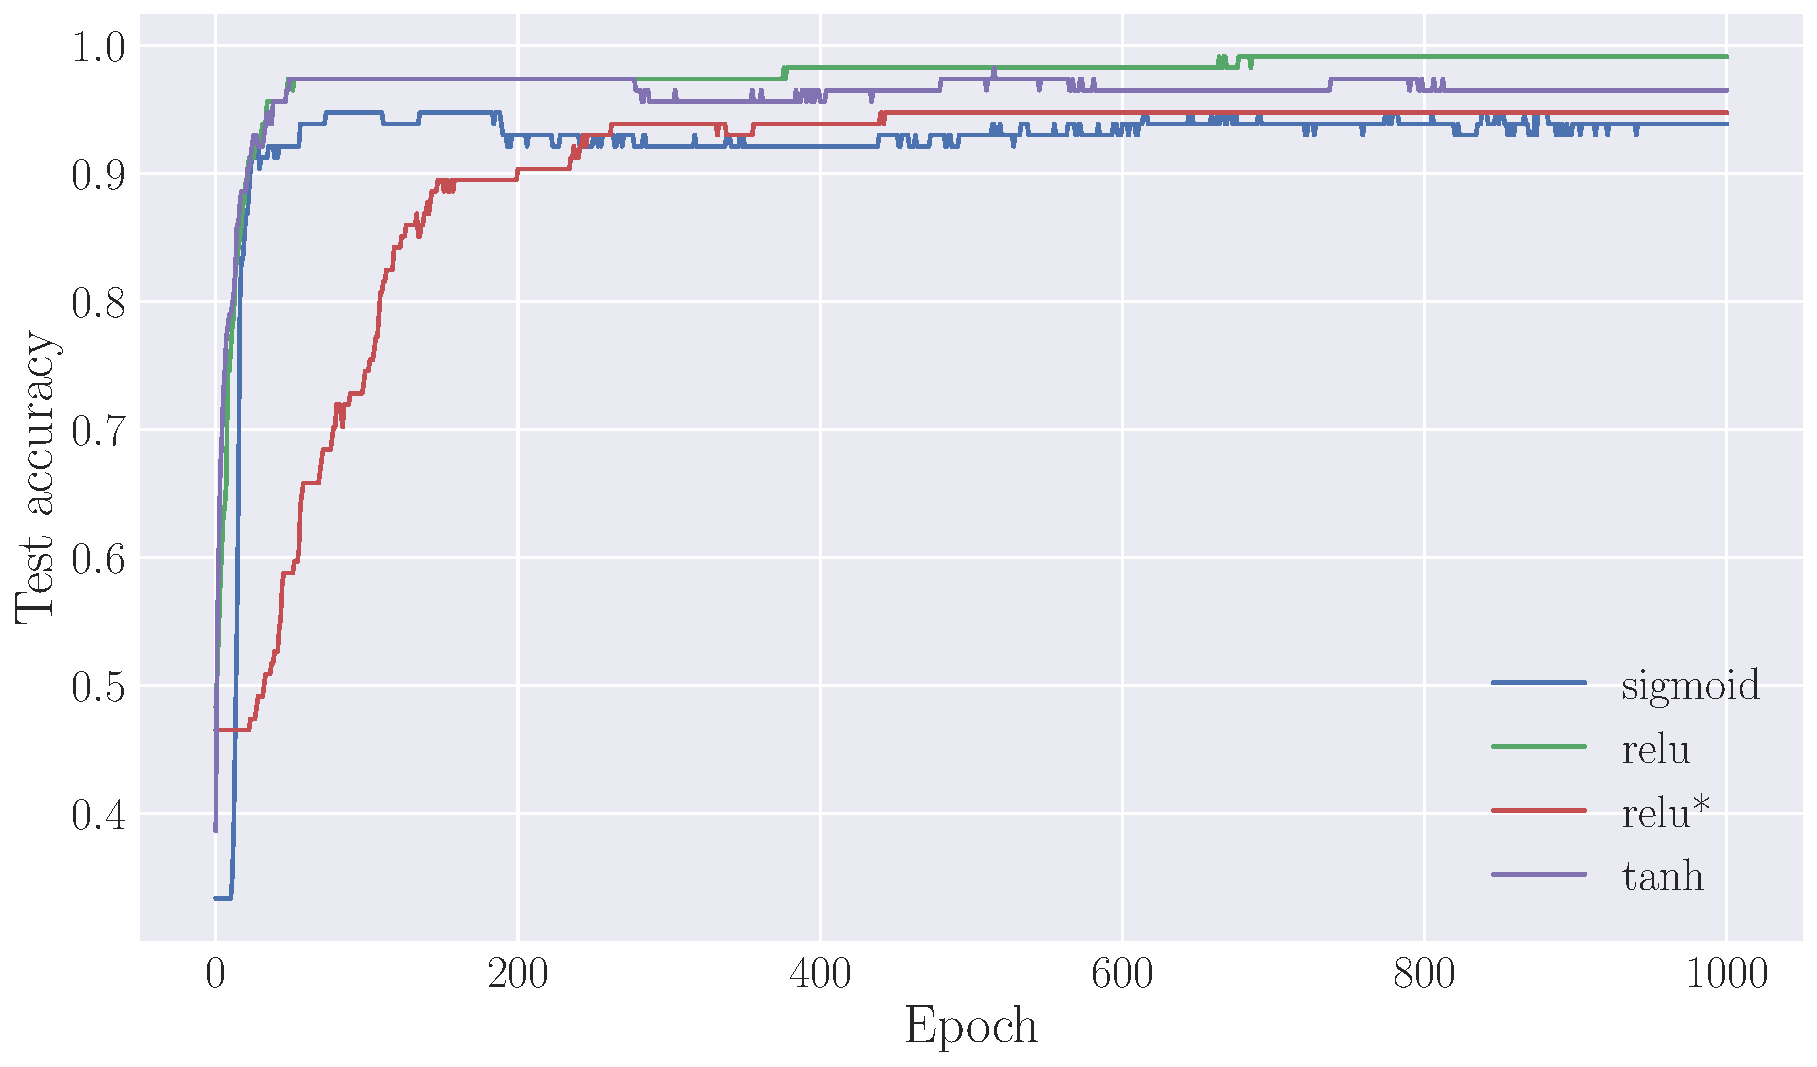
\includegraphics[width=\linewidth]{actFuncPerEpoch1000Cancer.pdf}
    \caption{Plot of accuracy for up to 1000 epochs, using SGD with RMSProp as optimiser performing regression analysis with $L-1=2$ hidden layers with $N_l=10$ neurons each with $\eta=10^{-3}$ and $\lambda=10^{-6}$. The four different activation functions perform differently.}
    \label{fig:class_act_epoch1000}
\end{figure}

\begin{figure}[h!]
    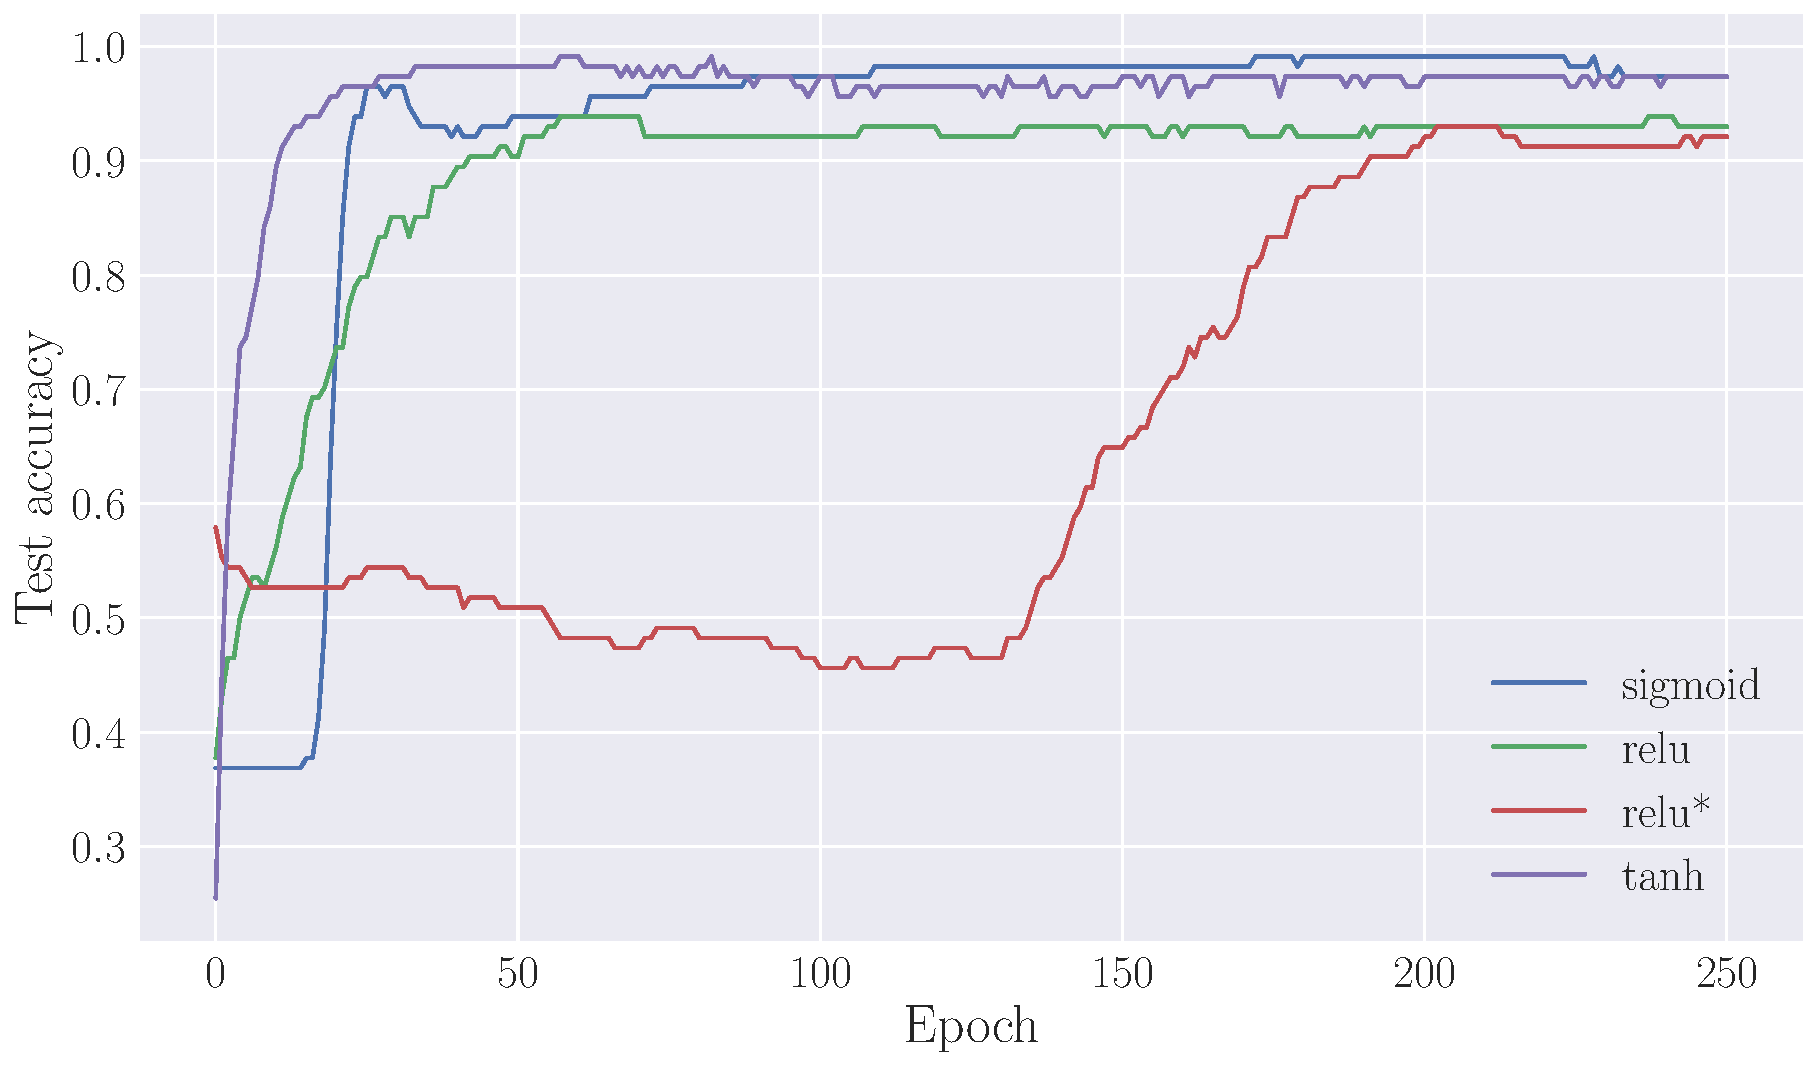
\includegraphics[width=\linewidth]{actFuncPerEpochCancer.pdf}
    \caption{Plot of accuracy for up to 250 epochs, using SGD with RMSProp as optimiser performing regression analysis with $L-1=2$ hidden layer with $N_l=10$ neurons with $\eta=10^{-3}$ and $\lambda=10^{-6}$. The four different activation functions perform differently.}
    \label{fig:class_act_epoch}
\end{figure}

\begin{figure}[h!]
    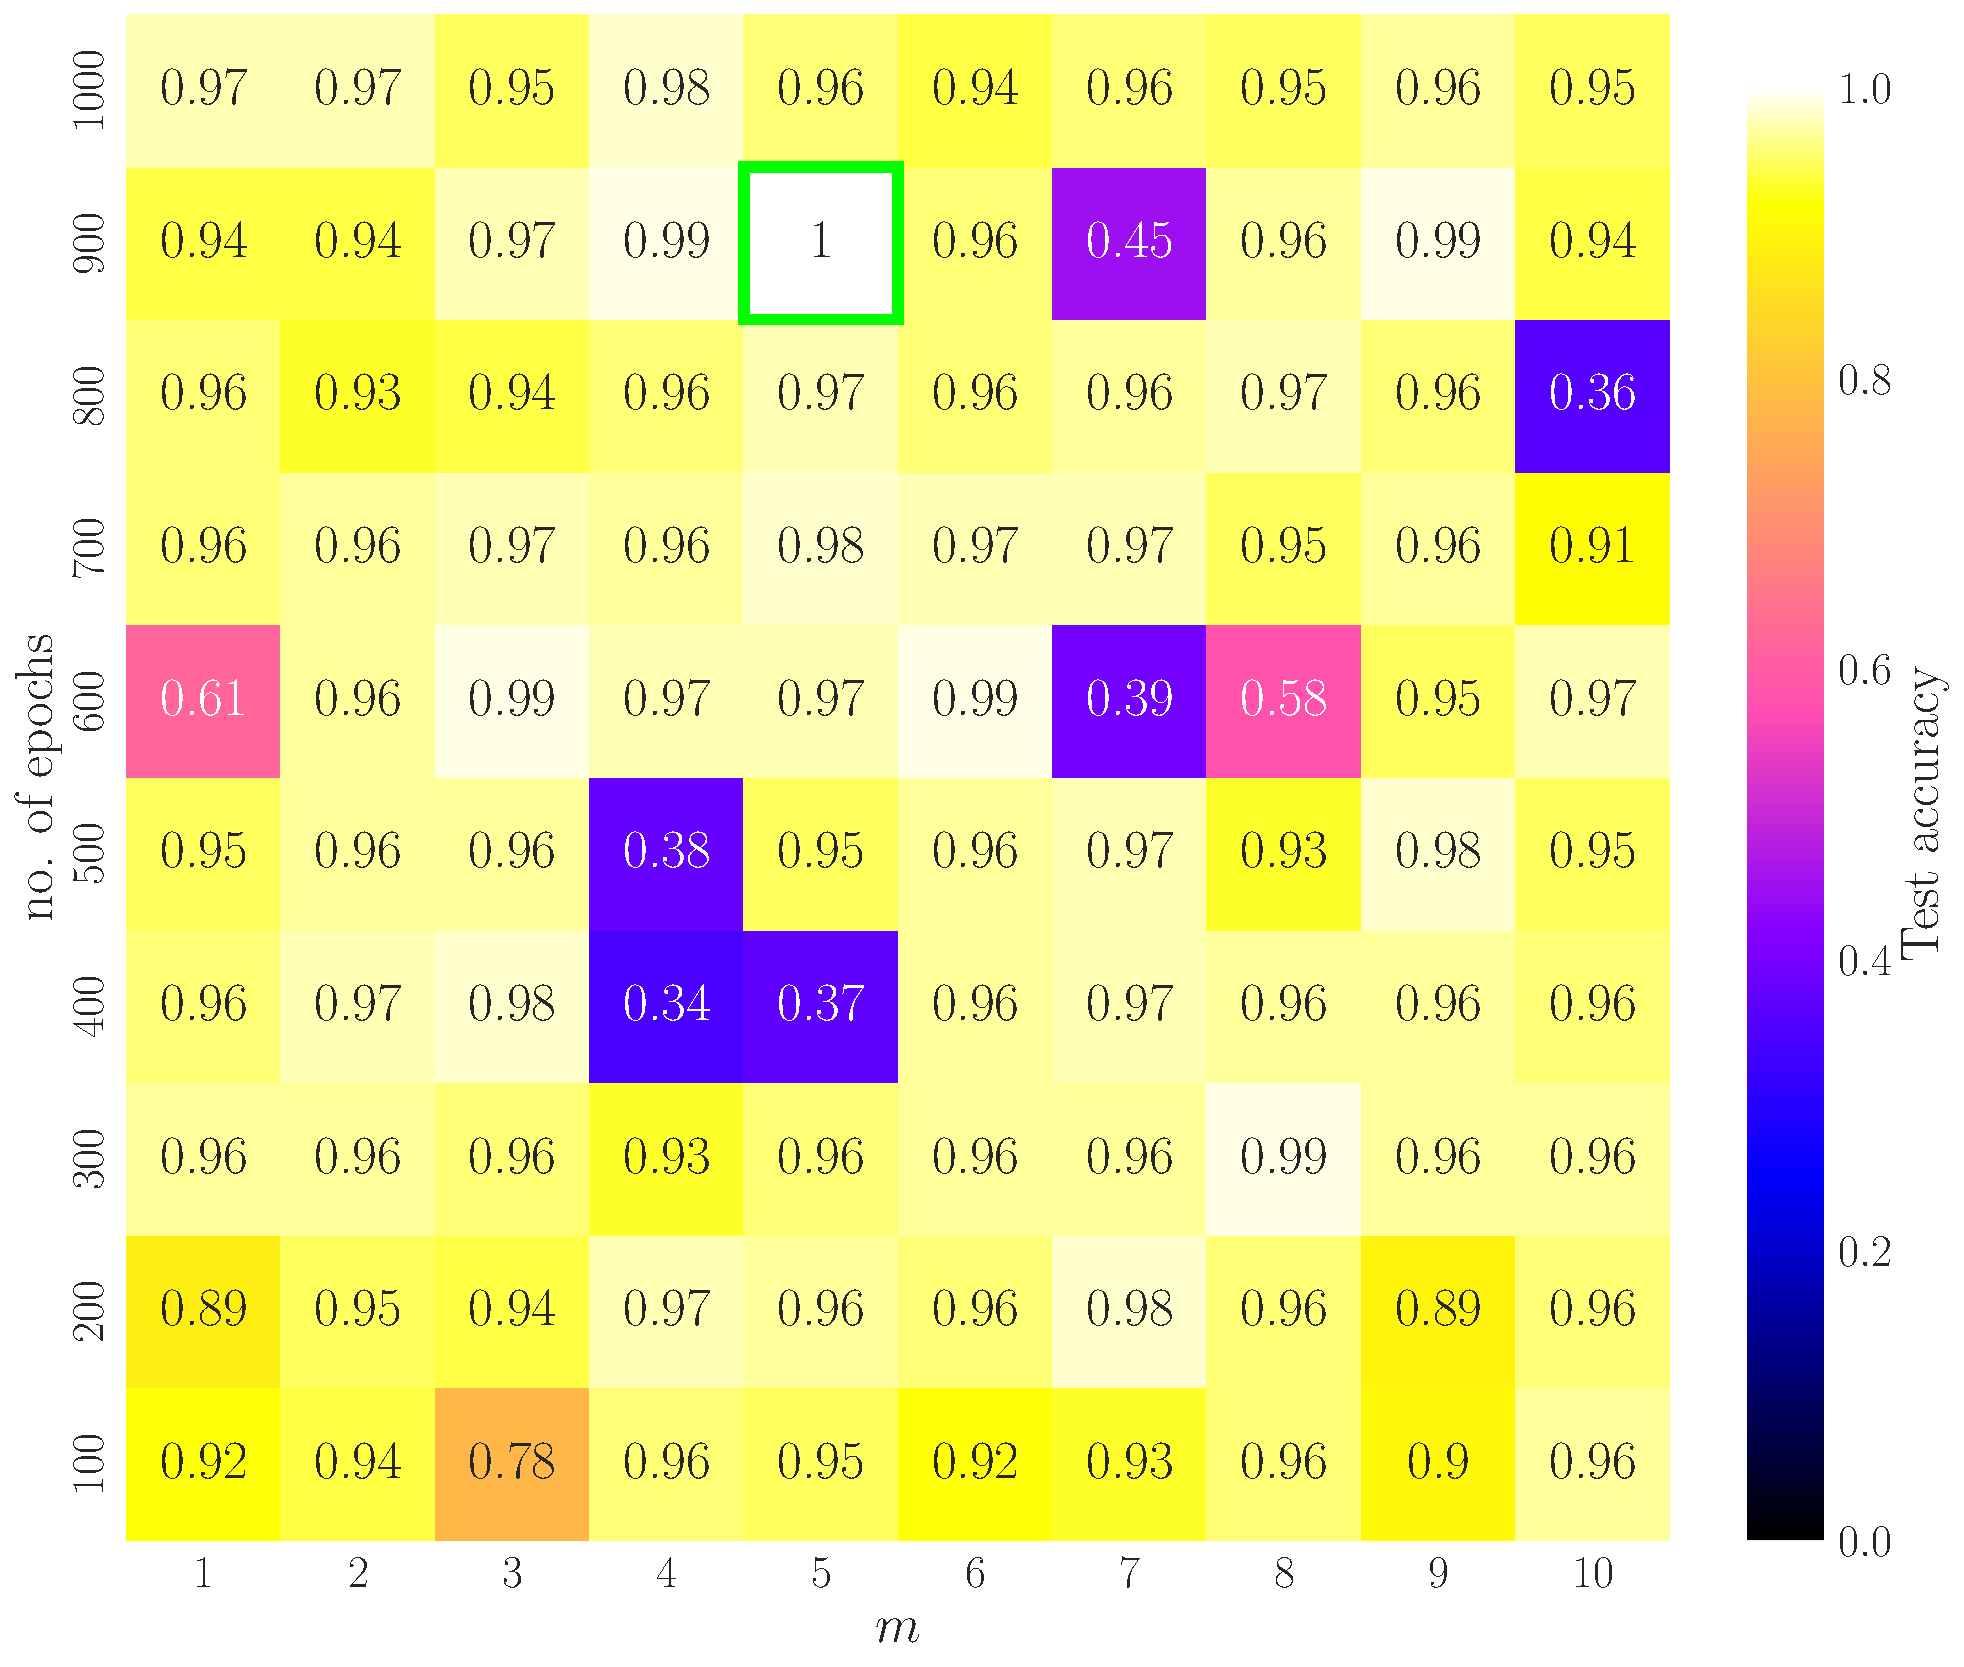
\includegraphics[width=\linewidth]{epoch_minibatch_analysisCancer.pdf}
    \caption{Heatmap of accuracy as function of the number of minibatches $m$ and training epochs, using SGD with RMSProp as optimiser performing regression analysis with $L-1=2$ hidden layer with $N_l=10$ neurons with $\eta=10^{-3}$ and $\lambda=10^{-6}$ using RELU as activation function. }
    \label{fig:class_minibatch_epoch}
\end{figure}


\clearpage

\section{Logistic regression figure}\label{app:logistic}

\begin{figure}[h!]
    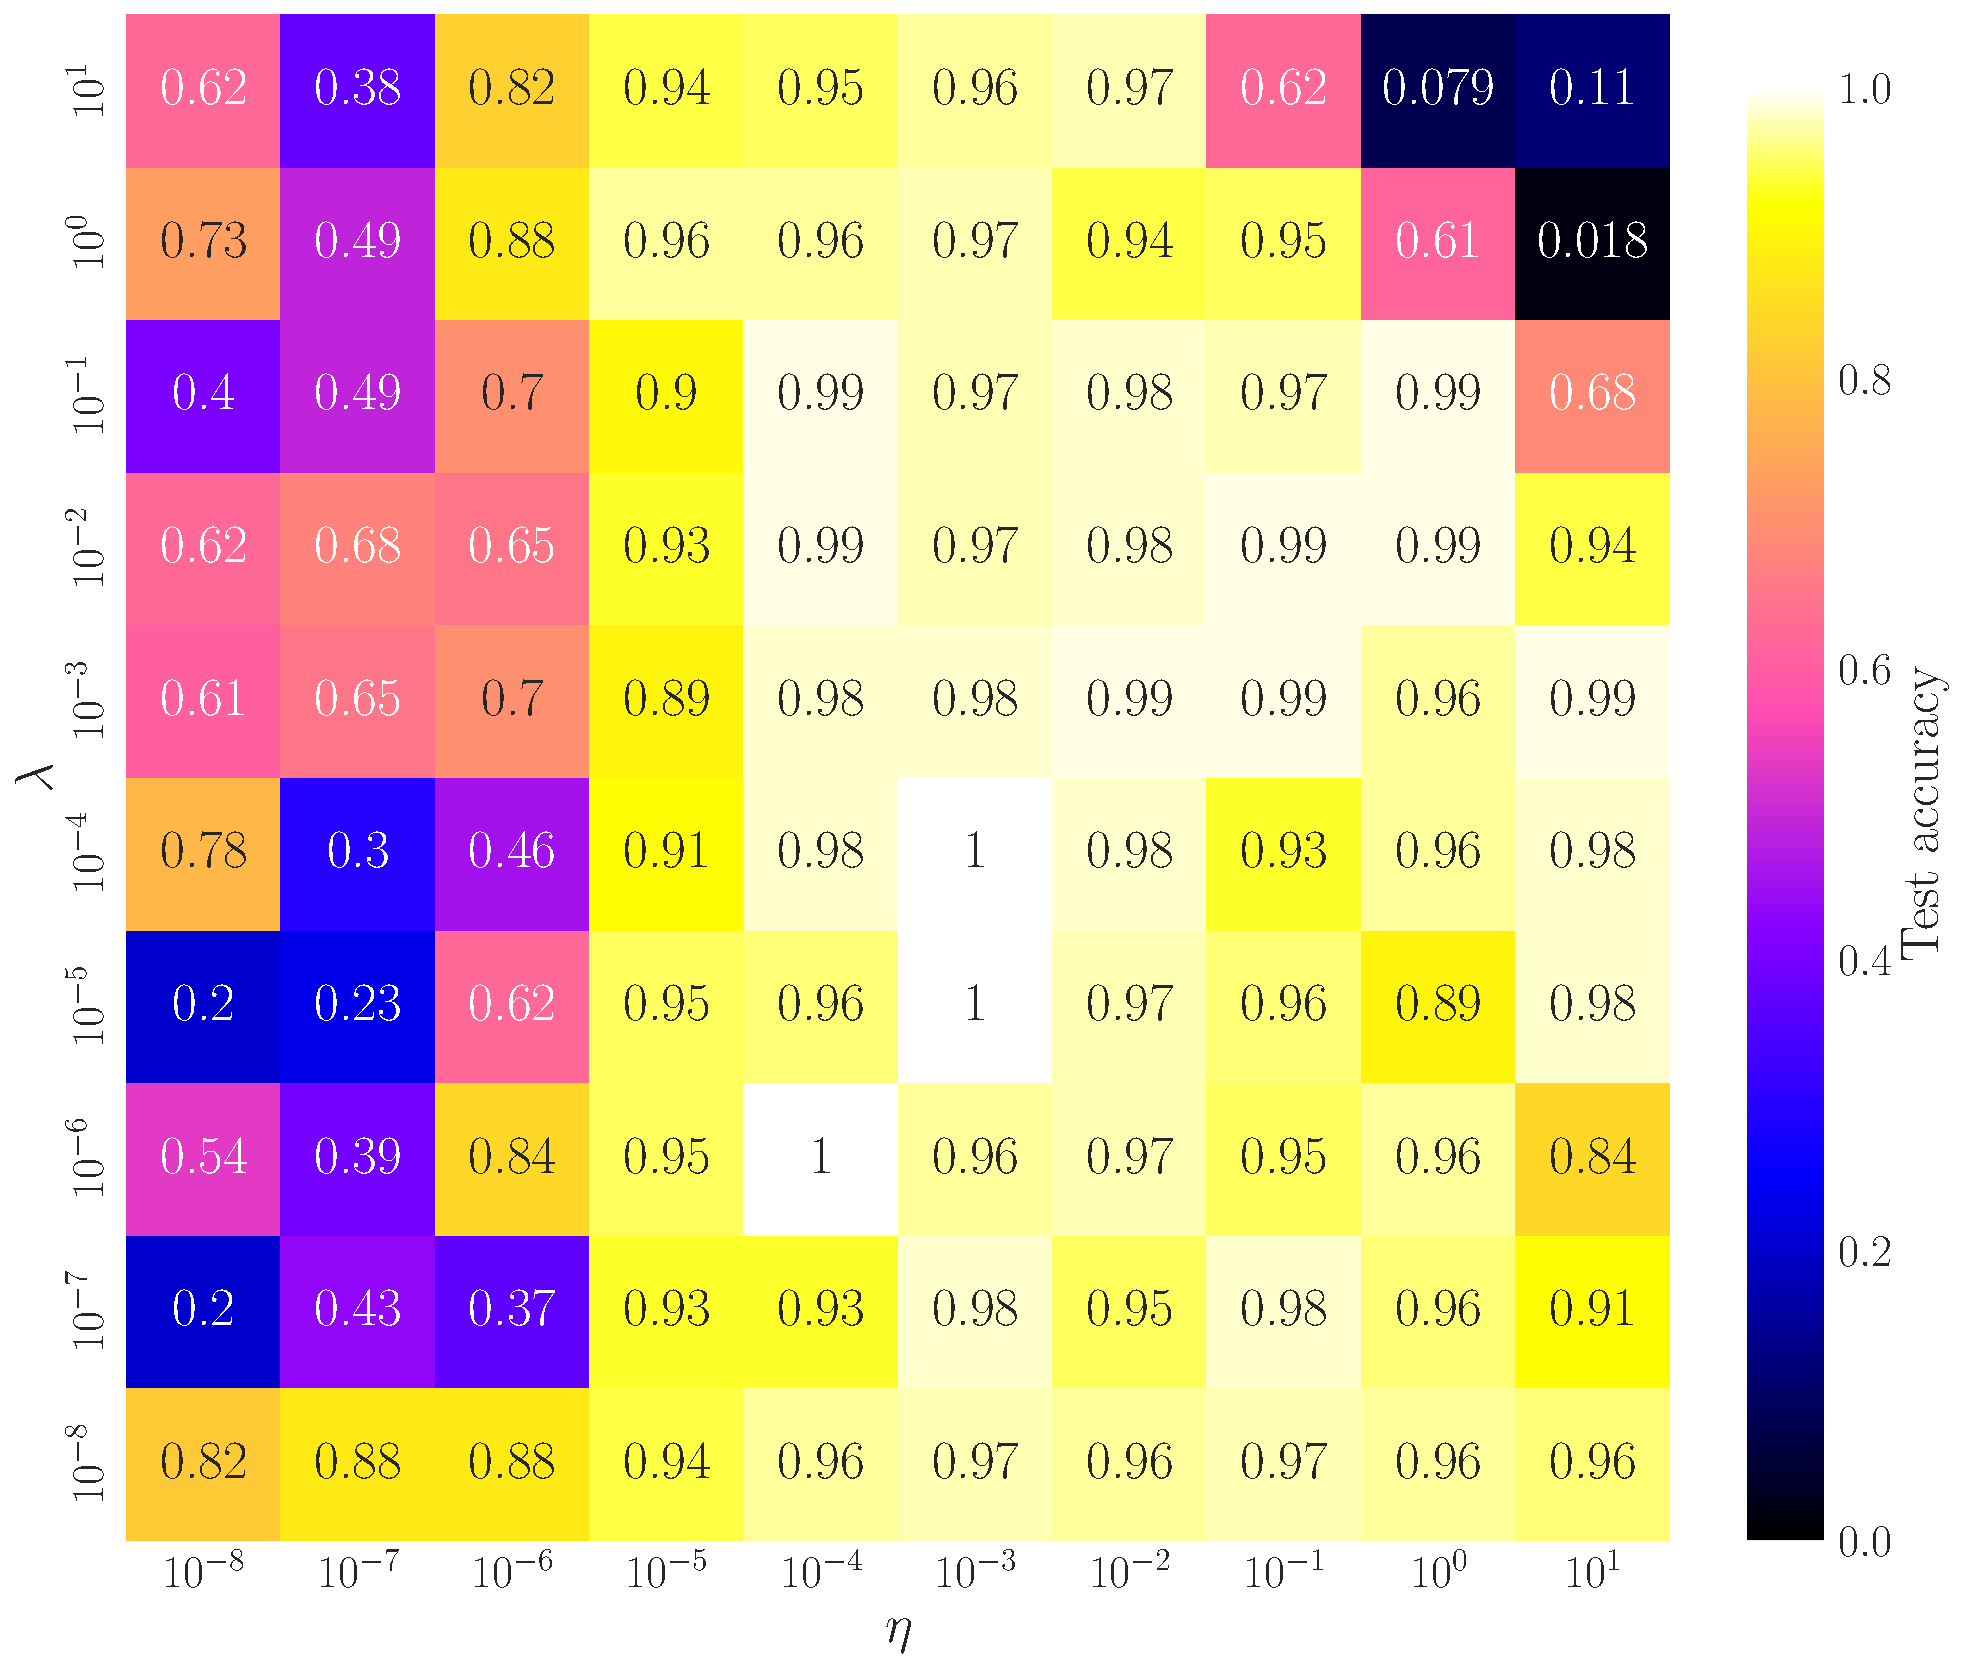
\includegraphics[width=\linewidth]{logistic.pdf}
    \caption{Heatmap of the MSE as function of learning rate $\eta$ and regularisation parameter $\lambda$, using SGD with RMSProp as optimiser performing regression analysis of a network with no hidden layers using the sigmoid function as activation function. This is equivalent of performing logistic regression.}
    \label{fig:logistic_eta_lambda}
\end{figure}
\end{document}
